\documentclass[
  man,
  longtable,
  nolmodern,
  notxfonts,
  notimes,
  colorlinks=true,linkcolor=blue,citecolor=blue,urlcolor=blue]{apa7}

\usepackage{amsmath}
\usepackage{amssymb}



\usepackage[bidi=default]{babel}
\babelprovide[main,import]{english}


% get rid of language-specific shorthands (see #6817):
\let\LanguageShortHands\languageshorthands
\def\languageshorthands#1{}

\RequirePackage{longtable}
\RequirePackage{threeparttablex}

\makeatletter
\renewcommand{\paragraph}{\@startsection{paragraph}{4}{\parindent}%
	{0\baselineskip \@plus 0.2ex \@minus 0.2ex}%
	{-.5em}%
	{\normalfont\normalsize\bfseries\typesectitle}}

\renewcommand{\subparagraph}[1]{\@startsection{subparagraph}{5}{0.5em}%
	{0\baselineskip \@plus 0.2ex \@minus 0.2ex}%
	{-\z@\relax}%
	{\normalfont\normalsize\bfseries\itshape\hspace{\parindent}{#1}\textit{\addperi}}{\relax}}
\makeatother




\usepackage{longtable, booktabs, multirow, multicol, colortbl, hhline, caption, array, float, xpatch}
\usepackage{subcaption}


\renewcommand\thesubfigure{\Alph{subfigure}}
\setcounter{topnumber}{2}
\setcounter{bottomnumber}{2}
\setcounter{totalnumber}{4}
\renewcommand{\topfraction}{0.85}
\renewcommand{\bottomfraction}{0.85}
\renewcommand{\textfraction}{0.15}
\renewcommand{\floatpagefraction}{0.7}

\usepackage{tcolorbox}
\tcbuselibrary{listings,theorems, breakable, skins}
\usepackage{fontawesome5}

\definecolor{quarto-callout-color}{HTML}{909090}
\definecolor{quarto-callout-note-color}{HTML}{0758E5}
\definecolor{quarto-callout-important-color}{HTML}{CC1914}
\definecolor{quarto-callout-warning-color}{HTML}{EB9113}
\definecolor{quarto-callout-tip-color}{HTML}{00A047}
\definecolor{quarto-callout-caution-color}{HTML}{FC5300}
\definecolor{quarto-callout-color-frame}{HTML}{ACACAC}
\definecolor{quarto-callout-note-color-frame}{HTML}{4582EC}
\definecolor{quarto-callout-important-color-frame}{HTML}{D9534F}
\definecolor{quarto-callout-warning-color-frame}{HTML}{F0AD4E}
\definecolor{quarto-callout-tip-color-frame}{HTML}{02B875}
\definecolor{quarto-callout-caution-color-frame}{HTML}{FD7E14}

%\newlength\Oldarrayrulewidth
%\newlength\Oldtabcolsep


\usepackage{hyperref}




\providecommand{\tightlist}{%
  \setlength{\itemsep}{0pt}\setlength{\parskip}{0pt}}
\usepackage{longtable,booktabs,array}
\usepackage{calc} % for calculating minipage widths
% Correct order of tables after \paragraph or \subparagraph
\usepackage{etoolbox}
\makeatletter
\patchcmd\longtable{\par}{\if@noskipsec\mbox{}\fi\par}{}{}
\makeatother
% Allow footnotes in longtable head/foot
\IfFileExists{footnotehyper.sty}{\usepackage{footnotehyper}}{\usepackage{footnote}}
\makesavenoteenv{longtable}

\usepackage{graphicx}
\makeatletter
\newsavebox\pandoc@box
\newcommand*\pandocbounded[1]{% scales image to fit in text height/width
  \sbox\pandoc@box{#1}%
  \Gscale@div\@tempa{\textheight}{\dimexpr\ht\pandoc@box+\dp\pandoc@box\relax}%
  \Gscale@div\@tempb{\linewidth}{\wd\pandoc@box}%
  \ifdim\@tempb\p@<\@tempa\p@\let\@tempa\@tempb\fi% select the smaller of both
  \ifdim\@tempa\p@<\p@\scalebox{\@tempa}{\usebox\pandoc@box}%
  \else\usebox{\pandoc@box}%
  \fi%
}
% Set default figure placement to htbp
\def\fps@figure{htbp}
\makeatother


% definitions for citeproc citations
\NewDocumentCommand\citeproctext{}{}
\NewDocumentCommand\citeproc{mm}{%
  \begingroup\def\citeproctext{#2}\cite{#1}\endgroup}
\makeatletter
 % allow citations to break across lines
 \let\@cite@ofmt\@firstofone
 % avoid brackets around text for \cite:
 \def\@biblabel#1{}
 \def\@cite#1#2{{#1\if@tempswa , #2\fi}}
\makeatother
\newlength{\cslhangindent}
\setlength{\cslhangindent}{1.5em}
\newlength{\csllabelwidth}
\setlength{\csllabelwidth}{3em}
\newenvironment{CSLReferences}[2] % #1 hanging-indent, #2 entry-spacing
 {\begin{list}{}{%
  \setlength{\itemindent}{0pt}
  \setlength{\leftmargin}{0pt}
  \setlength{\parsep}{0pt}
  % turn on hanging indent if param 1 is 1
  \ifodd #1
   \setlength{\leftmargin}{\cslhangindent}
   \setlength{\itemindent}{-1\cslhangindent}
  \fi
  % set entry spacing
  \setlength{\itemsep}{#2\baselineskip}}}
 {\end{list}}
\usepackage{calc}
\newcommand{\CSLBlock}[1]{\hfill\break\parbox[t]{\linewidth}{\strut\ignorespaces#1\strut}}
\newcommand{\CSLLeftMargin}[1]{\parbox[t]{\csllabelwidth}{\strut#1\strut}}
\newcommand{\CSLRightInline}[1]{\parbox[t]{\linewidth - \csllabelwidth}{\strut#1\strut}}
\newcommand{\CSLIndent}[1]{\hspace{\cslhangindent}#1}





\usepackage{newtx}

\defaultfontfeatures{Scale=MatchLowercase}
\defaultfontfeatures[\rmfamily]{Ligatures=TeX,Scale=1}





\title{The role of cognateness in native spoken word recognition}


\shorttitle{The role of cognateness in native spoken word recognition}


\usepackage{etoolbox}









\authorsnames[{1},{2},{2},{1}]{Gonzalo Garcia-Castro,Serene Siow,Kim
Plunkett,Nuria Sebastian-Galles}







\authorsaffiliations{
{Center for Brain and Cognition, Universitat Pompeu Fabra},{Department
of Experimental Psychology, University of Oxford}}




\leftheader{Garcia-Castro, Siow, Plunkett and Sebastian-Galles}



\abstract{When listening to speech in an unfamiliar language, words and
phrases in the native language are frequently activated due to their
acoustic similarity with some parts of the speech stream. This study
explored this phenomenon, for the first time, from a language processing
perspective. Across three studies, English- and Spanish-native adults
completed a translation elicitation task, in which they listened to a
series of words from an unfamiliar language (Catalan or Spanish for
English speakers, Catalan for Spanish speakers). For each presented
word, participants had to type their best-guess translation in their
native language. Both English and Spanish natives were surprisingly good
at translating unfamiliar words, efficiently exploiting the phonological
similarity between the presented (unfamiliar) words and their correct
translation. When the correct translation belonged to high-density
phonological neighbourhood, participants' ability to benefit from
phonological similarity decreased. Spanish participants, whose native
language was typologically closer to the presented language, benefited
more strongly from phonological similarity than English participants.
Overall, we show that speech in an unfamiliar language triggers
equivalent dynamics of lexical selection than native speech, providing a
psycholinguistic account for homophonic translation. }

\keywords{cognateness, spoken word recognition, phonology, speech
processing, non-native speech, lexical access}

\authornote{\par{\addORCIDlink{Gonzalo
Garcia-Castro}{0000-0002-8553-4209}}\par{\addORCIDlink{Serene
Siow}{0000-0001-6482-2191}}\par{\addORCIDlink{Kim
Plunkett}{0000-0003-0216-7480}}\par{\addORCIDlink{Nuria
Sebastian-Galles}{0000-0001-6938-2498}} 

\par{       }
\par{Correspondence concerning this article should be addressed
to Gonzalo
Garcia-Castro, Email: \href{mailto:gonzalo.garciadecastro@upf.edu}{gonzalo.garciadecastro@upf.edu}}
}

\makeatletter
\let\endoldlt\endlongtable
\def\endlongtable{
\hline
\endoldlt
}
\makeatother
\RequirePackage{longtable}
\DeclareDelayedFloatFlavor{longtable}{table}

\urlstyle{same}



\usepackage{booktabs}

\usepackage{caption}

\usepackage{longtable}

\usepackage{colortbl}

\usepackage{array}

\usepackage{float}

\usepackage{tabularray}

\usepackage[normalem]{ulem}

\usepackage{graphicx}

\UseTblrLibrary{booktabs}

\UseTblrLibrary{rotating}

\UseTblrLibrary{siunitx}

\NewTableCommand{\tinytableDefineColor}[3]{\definecolor{#1}{#2}{#3}}

\newcommand{\tinytableTabularrayUnderline}[1]{\underline{#1}}

\newcommand{\tinytableTabularrayStrikeout}[1]{\sout{#1}}

\makeatletter
\@ifpackageloaded{float}{}{\usepackage{float}}
\floatstyle{plain}
\@ifundefined{c@chapter}{\newfloat{apxfig}{h}{loapxfig}}{\newfloat{apxfig}{h}{loapxfig}[chapter]}
\floatname{apxfig}{Appendix Fig.}
\newcommand*\listofapxfigs{\listof{apxfig}{List of Appendix Fig.s}}
\makeatother
\makeatletter
\@ifpackageloaded{caption}{}{\usepackage{caption}}
\AtBeginDocument{%
\ifdefined\contentsname
  \renewcommand*\contentsname{Table of contents}
\else
  \newcommand\contentsname{Table of contents}
\fi
\ifdefined\listfigurename
  \renewcommand*\listfigurename{List of Figures}
\else
  \newcommand\listfigurename{List of Figures}
\fi
\ifdefined\listtablename
  \renewcommand*\listtablename{List of Tables}
\else
  \newcommand\listtablename{List of Tables}
\fi
\ifdefined\figurename
  \renewcommand*\figurename{Figure}
\else
  \newcommand\figurename{Figure}
\fi
\ifdefined\tablename
  \renewcommand*\tablename{Table}
\else
  \newcommand\tablename{Table}
\fi
}
\@ifpackageloaded{float}{}{\usepackage{float}}
\floatstyle{ruled}
\@ifundefined{c@chapter}{\newfloat{codelisting}{h}{lop}}{\newfloat{codelisting}{h}{lop}[chapter]}
\floatname{codelisting}{Listing}
\newcommand*\listoflistings{\listof{codelisting}{List of Listings}}
\makeatother
\makeatletter
\makeatother
\makeatletter
\@ifpackageloaded{caption}{}{\usepackage{caption}}
\@ifpackageloaded{subcaption}{}{\usepackage{subcaption}}
\makeatother

% From https://tex.stackexchange.com/a/645996/211326
%%% apa7 doesn't want to add appendix section titles in the toc
%%% let's make it do it
\makeatletter
\xpatchcmd{\appendix}
  {\par}
  {\addcontentsline{toc}{section}{\@currentlabelname}\par}
  {}{}
\makeatother

%% Disable longtable counter
%% https://tex.stackexchange.com/a/248395/211326

\usepackage{etoolbox}

\makeatletter
\patchcmd{\LT@caption}
  {\bgroup}
  {\bgroup\global\LTpatch@captiontrue}
  {}{}
\patchcmd{\longtable}
  {\par}
  {\par\global\LTpatch@captionfalse}
  {}{}
\apptocmd{\endlongtable}
  {\ifLTpatch@caption\else\addtocounter{table}{-1}\fi}
  {}{}
\newif\ifLTpatch@caption
\makeatother

\begin{document}

\maketitle




\setlength\LTleft{0pt}




\section{Introduction}\label{introduction}

When some German speakers listen to the song \emph{The Power} by SNAP!
(\emph{Coyote Ugly}, 2000), many of them mishear the line ``I've got the
power'' as \emph{Agatha Bauer}. When Spanish speakers listen to the line
``Circumvent your thick ego'' from the song \emph{Pictures} by System of
a Down (\emph{Steal this Album!}, 2002), they tend to hear \emph{Sácame
de aquí, King-Kong} {[}take me out of here, King-Kong{]}. Outrageous as
these examples might sound, the reader may know a few cases in their own
native language. This auditory illusion is common across languages and
cultures and can feel quite real, often inevitable
(\citeproc{ref-dembeck2015oberflachenubersetzung}{Dembeck, 2015};
\citeproc{ref-efimova2018homophonic}{Efimova et al., 2018}). In
Japanese, this phenomenon takes the name \emph{Soramimi} (lit. ``empty
ear''). From a linguistic point of view, Soramimi is a particular case
of homophonic translation: words or phrases that appear in the speech
stream in one language are translated into similar-sounding words and
phrases in a different language, without necessarily preserving the
meaning (\citeproc{ref-gasparov2006semen}{Gasparov, 2006}). Homophonic
translation has mostly received attention as a perceptual curiosity, and
as a literary figure, intentionally employed by translators to preserve
the meter and ``sound structure'' (e.g., rhymes) of an original text in
the language of translation (e.g.,
\citeproc{ref-levick2016translating}{Levick, 2016};
\citeproc{ref-pilshchikov2016semiotics}{Pilshchikov, 2016})\footnote{The
  rationale behind this translation approach is to ``sacrifice{[}s{]}
  fidelity to the image rather than the melodiousness of verse''
  (\citeproc{ref-briusov1911ot}{Briusov, 1911}). For instance, Edith
  Grossman's translation of \emph{El Quijote}
  (\citeproc{ref-cervantes}{Cervantes \& Grossman, 2002}) present a
  similar case, in which formal aspects of the original text in Spanish
  are favoured to some degree over equivalence to English, even
  sometimes keeping Spanish words from the original text in the English
  translation (e.g., \emph{Señor}, \emph{ínsula}).}. Little attention
has been paid to homophonic translation from a language processing
perspective.

One exception is the study by Otake
(\citeproc{ref-otake2007interlingual}{2007}), who analysed 194 instances
of Soramimi, broadcasted between 1992 and 2007 by the Japanese TV show
\emph{Soramimi hour}, in which examples of Soramimi were presented to
the audience for comedy purposes. These instances consisted of
homophonic translations of English song lyrics to words and phrases in
Japanese. The vast majority of the reported instances were phrases
(96\%) and a few, single words (4\%). There was relatively high
variability in the degree to which phonetic features of the presented
English lyrics were preserved, with some resulting Japanese words or
phrases sharing high overlap with the original English strings of
sounds, and some sharing very little overlap. An analysis of the few
instances of homophonic translations of single words revealed three main
phonological processes that could explain how Japanese listeners
reconstructed the English input to generate the Japanese words:
insertion (e.g., \emph{cry} /\textipa{kraI}/ to \emph{kurai}
/\textipa{kuRai}/ {[}dark{]}), deletion (e.g., \emph{go} /\textipa{goU}/
to \emph{go} /go/ {[}\emph{Go}, a board game{]}, and alternation (e.g.,
\emph{low} /\textipa{loU}/ to \emph{rou} /\textipa{Roo}/ {[}wax{]}).
This suggests that the reported homophonic translations can be
explained, to some extent, as the result of the Japanese listeners
accommodating the strings of English sounds to the Japanese phoneme
inventory and Japanese phonotactics
(\citeproc{ref-dupoux1999epenthetic}{Dupoux et al., 1999};
\citeproc{ref-peperkamp2008perceptual}{Peperkamp et al., 2008}).

The phonological processes described by Otake
(\citeproc{ref-otake2007interlingual}{2007}) do not take place in a
vaccum, but rather in the context of a lexicon. As words or phrases in
the native lexicon are activated by their acoustic similarity with the
non-native speech stream, they trigger a series of mechanisms that
result in the selection of one of the candidate word or phrase in the
native language. In the present work, we investigated the interplay
between phonological similarity and one of the main mechanisms involved
in the dynamics of lexical selection: phonological neighbourhood
density. The phonological neighbourhood density of a given word-form
refers to the number of words-forms that differ in a single phoneme from
the it. For instance, the English word \emph{cat} belongs to a dense
phonological neighbourhood, with 50 English phonological neighbours
(e.g., hat, bat, cap), while the word \emph{charger} belongs to a sparse
phonological neighbourhood, with six neighbours (e.g., charged, larger,
charter, charmer) (\citeproc{ref-marian2012clearpond}{Marian et al.,
2012}). Phonological neighbourhood density affects lexical processing.
For instance, words from dense neighbourhoods are recognized more slowly
and less accuractely in the auditory modality than words from sparse
neighbourhoods (\citeproc{ref-luce1998recognizing}{Luce \& Pisoni,
1998}; \citeproc{ref-vitevitch1998words}{Vitevitch \& Luce, 1998}; e.g.,
\citeproc{ref-dufour2010phonological}{Dufour \& Frauenfelder, 2010};
\citeproc{ref-vitevitch2006clustering}{M. Vitevitch, 2006}). In this
study, we examined how listeners may activate lexical representations in
their native language when listening to an unfamiliar language.

Although homophonic translations rarely involve preservation of meaning,
they sometimes lead to correct translations. For example, imagine an
English native listening to Dutch for the first time. This listener may
encounter the word /\textipa{"pINgUIn}/ (\emph{pinguin}), which sounds
similar to its English translation /\textipa{"pENgwIn}/ (penguin). Given
enough phonological similarity between the non-native word and its
translation in the native language, a naïve listener may succeed at word
comprehension when listening to an unfamiliar language. Such
phonological similarity between translation equivalents---known as
\emph{cognateness}---is common across many languages, and is often due
to typological closeness and/or socio-historical events involving the
speakers of these languages (e.g., migration, social contact). For
example, Romance languages such as Spanish and Catalan share many
form-similar translation equivalents
(\citeproc{ref-schepens2012distributions}{Schepens et al., 2012}), as in
the case of \emph{puerta} and \emph{porta} (\emph{door} in Spanish and
Catalan, respectively). Given no prior knowledge of either language, a
Spanish native speaker is likely to be much more successful at correctly
translating Catalan \emph{porta} than English \emph{door}, due to the
phonological and (orthographic similarity) of the former to the
equivalent in their native language.

To explore the lexical mechanisms triggered by unfamiliar speech
listening, we used a translation elicitation task in which participants
listened to words from an unfamiliar language, and then tried to guess
the words translations in their native language. We will henceforth
refer to the auditory-presented words heard by participants on each
trial as \emph{presented words}, and the correct translation for the
presented words as \emph{target translations}. By manipulating the
amount of phonological similarity between the presented words and their
target translations, we explored listeners' reliance on phonological
similarity to succeed in the task. Since participants were unfamiliar
with the presented language, they could only use phonological similarity
between the presented language and their native language to successfully
translate the words. We therefore predicted that participants'
performance should increase when the translation pairs are
phonologically more similar. We also predicted that there is a minimum
threshold of phonological similarity to be sufficient for correct
translation.

We further investigated the effect of phonological competition. Even if
the presented word and its target translation share high phonological
similarity, participants may still provide incorrect translations if the
presented word also shares high phonological similarity with other words
in the native language. Words with denser phonological neighbourhoods
are recognised more slowly and less accurately than words with sparser
phonological neighbourhoods (\citeproc{ref-dufour2003lexical}{Dufour \&
Peereman, 2003}; \citeproc{ref-goldinger1989priming}{Goldinger et al.,
1989}; \citeproc{ref-hamburger1996phonological}{Hamburger \& Slowiaczek,
1996}; \citeproc{ref-luce1990similarity}{Luce et al., 1990};
\citeproc{ref-luce1998recognizing}{Luce \& Pisoni, 1998}). This is
especially true if such neighbours share higher phonological similarity
with the presented word, or are lexically more frequent than the target
word (\citeproc{ref-luce1998recognizing}{Luce \& Pisoni, 1998}). Such
interference effect of phonological neighbourhood density has also been
reported across languages (\citeproc{ref-weber2004lexical}{Weber \&
Cutler, 2004}). We hypothesised that the size of the facilitatory role
of phonological similarity would be inversely proportional to the amount
of higher-frequency phonological neighbours of the presented word in the
target language. In the case of non-native speech recognition, the
presence of cross-linguistic pairs which are phonologically similar but
differ in meaning (e.g., false friends) may act as distractors during
lexical access, obstructing the selection of the appropriate target
translation in the listener's lexicon. For instance, Otwinowska and
Szewczyk (\citeproc{ref-otwinowska2019more}{2019}) reported that false
friends were disadvantaged relative to non-cognates by Polish second
language learners, in contrast to cognates which were known better. It
is therefore important to investigate the joint effect of both cognates
and false friends when investigating the effect that cross-linguistic
phonological similarity has on word recognition in a foreign language.
This could shed light on available strategies and challenges associated
with the early stages of second language acquisition. For instance, one
might expect English participants to incorrectly translate the Spanish
word \emph{botón} as \emph{bottom} instead of as its correct translation
\emph{button}, due to the combined effect of the close phonological
similarity between \emph{botón} and \emph{bottom} along with the high
lexical frequency of \emph{bottom} relative to \emph{button}. To test
this prediction, we developed a lexical frequency-dependent measure of
cross-language phonological neighbourhood density, in which a neighbour
is counted only if it is higher frequency and is one phoneme apart from
the presented word. If the phonological neighbourhood density of the
target translation affects participants' performance negatively, this
would suggest that competitors in the native language affect recognition
of non-native words during recognition of foreign speech. We conducted a
series of three experiments to test these predictions.

In Experiment 1, we collected data from two groups of British English
natives living in the United Kingdom. One group was presented with
Catalan words, the other with Spanish words. We examined the extent to
which participants were able to use the phonological similarity between
the presented word (in Catalan or Spanish) and its target translation to
provide accurate responses. In Experiment 2, we tested a group of
(European) Spanish natives in the same task, who were presented with
Catalan words. Catalan and Spanish are two Romance languages whose close
typological distance is reflected in the fact that they share many
cognates, where English is a Germanic language that shares considerably
fewer cognates with Catalan and Spanish. By testing participants
translating words from typologically close or distant languages, we
expected to widen the range of the phonological similarity scores of the
translation pairs involved in the experimental task, therefore allowing
us to explore potential cross-language differences in participant's
performance. One unexpected finding was that participants in Experiments
1 and 2 were surprisingly good at translating a subset of words which
had low phonological similarity with their correct translation. We were
concerned that this may be caused by some prior knowledge of specific
words by our participants, as some Spanish words are commonly seen in
media or product labels, making them familiar even to monolingual
speakers of English. In Experiment 3, we collected additional data from
a new group of British English natives. The design was closely modelled
after Experiment 1, except that after providing their response in each
trial, participants reported whether they had previous knowledge of the
presented word. In the final section of this article, we present
analyses on the joint data sets of Experiments 1 to 3.

\section{Experiment 1}\label{experiment-1}

\subsection{Methods}\label{methods}

All materials, data, and code used in this study are hosted in the Open
Science Framework
\href{https://osf.io/9fjxm/?view_only=aab7636ce1af48cf832596a7ea9101c5/}{https://osf.io/9fjxm/}
and a GitHub repository
\url{https://github.com/gongcastro/translation-elicitation.git}, along
with additional notes. For reproducibility, a Docker image of the
RStudio session is available on DockerHub
(\url{https://hub.docker.com/repository/docker/gongcastro/translation-elicitation/general}).

\subsubsection{Participants}\label{participants}

We collected data from 71 British English-native adults living in the
United Kingdom (\emph{Mean} = 21.76 years, \emph{SD} = 2.15, Range =
18-26, 46 female). Data collection took place from June 4th, 2020 to
June 25th, 2020. Participants were recruited via Prolific (£5
compensation) and SONA (compensation in academic credits). Participants
gave informed consent before providing any data. The study was conducted
in accordance with ethical standards of the Declaration of Helsinki and
the protocol was by the University of Oxford Medical Sciences
Inter-Divisional Research Ethics Committee (IDREC) (R60939/RE007).
Participants were asked to complete the experiment using a laptop in a
quiet place with good internet connection.

\begin{table}

{\caption{{Participant details.}{\label{tbl-participants}}}
\vspace{-20pt}}

\setlength{\LTpost}{0mm}
\begin{longtable*}{l|rrrc}
\toprule
\multicolumn{1}{l}{} &  & \multicolumn{2}{c}{Age} &  \\ 
\cmidrule(lr){3-4}
\multicolumn{1}{l}{} & N\textsuperscript{\textit{1}} & Mean ± SD  & Range & Second language \\ 
\midrule\addlinespace[2.5pt]
\multicolumn{5}{l}{Experiment 1} \\ 
\midrule\addlinespace[2.5pt]
spa-ENG & 35 (8) & $21.80$ ± $2.08$ & $18$–$26$ & Russian (1) \\ 
cat-ENG & 36 (4) & $21.72$ ± $2.25$ & $18$–$25$ & French (1), German (1), Italian (1), Punjabi (1), Several (1) \\ 
\midrule\addlinespace[2.5pt]
\multicolumn{5}{l}{Experiment 2} \\ 
\midrule\addlinespace[2.5pt]
cat-SPA & 33 (12) & $21.85$ ± $3.00$ & $18$–$33$ & French (9), German (1), Italian (2) \\ 
\midrule\addlinespace[2.5pt]
\multicolumn{5}{l}{Experiment 3} \\ 
\midrule\addlinespace[2.5pt]
spa-ENG & 32 (1) & $21.72$ ± $2.59$ & $18$–$26$ & German (2), Japanese (1) \\ 
cat-ENG & 32 (0) & $22.31$ ± $2.39$ & $18$–$26$ & Cantonese (1), Irish (1) \\ 
\bottomrule
\end{longtable*}
\begin{minipage}{\linewidth}
\textsuperscript{\textit{1}}Number of included participants (number of excluded participants.)\\
\end{minipage}

\end{table}

\subsubsection{Stimuli}\label{stimuli}

We created two lists of words to be presented to participants in the
auditory modality: one in Catalan and one in Spanish. Words in the
Catalan list were 6.67 phonemes long on average (\emph{SD} = 2.06, Range
= 2-11), and the orthographic forms of their English translations (which
participants had to type) were 5.12 characters long on average
(\emph{SD} = 1.56, Range = 3-9). Words in the Spanish list were 7.27
phonemes long on average (\emph{SD} = 2.05, Range = 3-13), and the
orthographic form of their English translations were 5.29 characters
long on average (\emph{SD} = 1.77, Range = 3-12).

In each trial, participants listened to one audio file, which contained
a single word. The audio files were the same ones used in child
experiments conducted in the Laboratori de Recerca en Infància of
Universitat Pompeu Fabra (Barcelona, Spain). These audio files were
recorded by a proficient Catalan-Spanish female bilingual from the
Metropolitan Area of Barcelona in a child-directed manner. Catalan and
Spanish words were recorded at 44,100 Hz in separate files in the same
session, and then de-noised using Audacity and normalised at peak
intensity using Praat (\citeproc{ref-broersma2021praat}{Broersma \&
Weenink, 2021}). The average duration of the Catalan audio files was
1.24 seconds (\emph{SD} = 0.19, Range = 0.8-1.58). The average duration
of the Spanish audio files was 1.16 seconds (\emph{SD} = 0.15, Range =
0.78-1.53).

For each word pair in the Catalan and Spanish lists, we defined three
predictors of interest: the lexical frequency of the correct English
translation (\emph{Frequency}), the phonological similarity between the
presented word and its correct English translation (\emph{Similarity}),
and the presented word's number of cross-language phonological
neighbours (\emph{CLPN}) in English. \emph{Frequency} was included as a
nuisance predictor, under the hypothesis that---keeping other predictors
constant---participants would provide correct responses more often when
the correct translations are high frequency words in their native
language. Lexical frequencies of correct translations were extracted
from SUBTLEX-UK (\citeproc{ref-van2014subtlex}{Van Heuven et al.,
2014}), and transformed to Zipf scores. Translations without a lexical
frequency value were excluded from data analysis (2 in the Catalan list,
5 in the Spanish list). \emph{Similarity}, our main predictor of
interest, was calculated as the Levenshtein similarity between the
X-SAMPA transcriptions of each pair of translations using the
\texttt{stringdist} R package (\citeproc{ref-van2014stringdist}{van der
Loo, 2014}). The Levenshtein distance computes the edit distance between
two character strings---in this case, two phonological
transcriptions---by counting the number of additions, deletions, and
substitutions necessary to make both strings identical
(\citeproc{ref-levenshtein1966binary}{Levenshtein, 1966}). We divided
this edit distance by the number of characters in the longest X-SAMPA
transcription of the translation pair. This transformation accounts for
the fact that Levenshtein distance tends to increase with the length of
the transcriptions. For interpretability, we subtracted this proportion
from one, so that values closer to one correspond to higher similarity
between phonological transcriptions, and values closer to zero
correspond to lower similarity between phonological transcriptions. For
example, the \emph{table} (\texttt{teIb@l})-\emph{mesa} (\texttt{mesa})
translation pair had 17\% similarity, while the \emph{train}
(\texttt{trEIn})-\emph{tren} (\texttt{tREn}) translation pair had 60\%
similarity. We calculated the number of \emph{CLPN} for each Catalan and
Spanish word by counting the number of English words with same or higher
lexical frequency, and whose phonological transcription (in X-SAMPA
format) differed by up to one phoneme from that of the presented Catalan
or Spanish word. Lexical frequencies and phonological transcriptions
were extracted from the multilingual database CLEARPOND
(\citeproc{ref-marian2012clearpond}{Marian et al., 2012})\footnote{Phonological
  transcriptions in CLEARPOND were generated from eSPEAK,
  \url{http://espeak.sourceforge.net/}}{]}. Table~\ref{tbl-stimuli}
summarises the lexical frequency, \emph{CLPN} and phonological overlap
of the words included in the Catalan and the Spanish lists.

\begin{table}

{\caption{{Stimuli details.}{\label{tbl-stimuli}}}
\vspace{-20pt}}

\begin{longtable*}{l|rrrrrr}
\toprule
\multicolumn{1}{l}{} & \multicolumn{2}{c}{Frequency} & \multicolumn{2}{c}{Similarity} & \multicolumn{2}{c}{CLPN} \\ 
\cmidrule(lr){2-3} \cmidrule(lr){4-5} \cmidrule(lr){6-7}
\multicolumn{1}{l}{} & Mean ± SD & Range & Mean ± SD & Range & Mean ± SD & Range \\ 
\midrule\addlinespace[2.5pt]
spa-ENG & $5.88$ ± $0.57$ & $4.43$–$7.24$ & $0.13$ ± $0.18$ & $0.00$–$0.75$ & $0.19$ ± $0.79$ & $0$–$5$ \\ 
cat-ENG & $5.89$ ± $0.59$ & $4.43$–$7.27$ & $0.16$ ± $0.18$ & $0.00$–$0.67$ & $0.76$ ± $2.53$ & $0$–$15$ \\ 
cat-SPA & $5.79$ ± $0.63$ & $4.48$–$7.70$ & $0.38$ ± $0.26$ & $0.00$–$1.00$ & $0.87$ ± $2.08$ & $0$–$12$ \\ 
\midrule 
\midrule 
\textbf{Mean} & $5.85$ & — & $0.225$ & — & $0.606$ & — \\ 
\bottomrule
\end{longtable*}

\end{table}

\subsubsection{Procedure}\label{procedure}

The experiment was implemented online using Psychopy/Pavlovia
(\citeproc{ref-peirce2019psychopy2}{Peirce et al., 2019}). Participants
accessed the study from a link provided by Prolific or SONA and
completed the experiment from an internet browser (Chrome or Mozilla).
After giving their consent for participating, participants answered a
series of questions about their demographic status, their language
background, and the set up they were using for completing the study.
Then, participants completed the experimental task. Participants were
informed that they would listen to a series of pre-recorded words in
either Catalan or Spanish. They were instructed to listen to each word,
guess its meaning in English, and type their answer as soon as possible.
Participants were randomly assigned to the Catalan or Spanish lists.
Participants in the Catalan list were presented with 83 trials, and
participants in the Spanish list were presented with 99
trials\footnote{Stimuli lists were built from a pool of audio recordings
  made for a different study. The different number of trials in the
  Catalan and Spanish lists is due to more Spanish audios being
  available than Catalan audios.}.

Each trial started with a yellow fixation point presented during one
second on the centre of the screen over a black background. After one
second, the audio started playing while the dot remained being displayed
until the audio ended. Upon the offset of the fixation point and audio,
participants were prompted to write their answer by a
\texttt{\textgreater{}} symbol. Typed letters were displayed on the
screen in real time to provide visual feed-back to participants.
Participants were allowed to correct their answer. Then, participants
pressed the \texttt{RETURN/ENTER} key to confirm their answer and start
a new trial. Figure~\ref{fig-design} illustrates the time course of a
trial in the translation elicitation task.

\begin{figure}

\caption{\label{fig-design}Schematic representation of a trial in the
experimental task. The trial stars with the presentation of a fixation
point in the centre of the screen (yellow dot). After 1,000 ms, the
auditory word was presented while the fixation point remained on screen.
After the offset of the audio, the fixation point disappeared and a
visual prompt (\texttt{\textgreater{}}) was presented. Participants then
wrote their answer and clicked \texttt{RETURN}, making the end of the
trial.}

\centering{

\pandocbounded{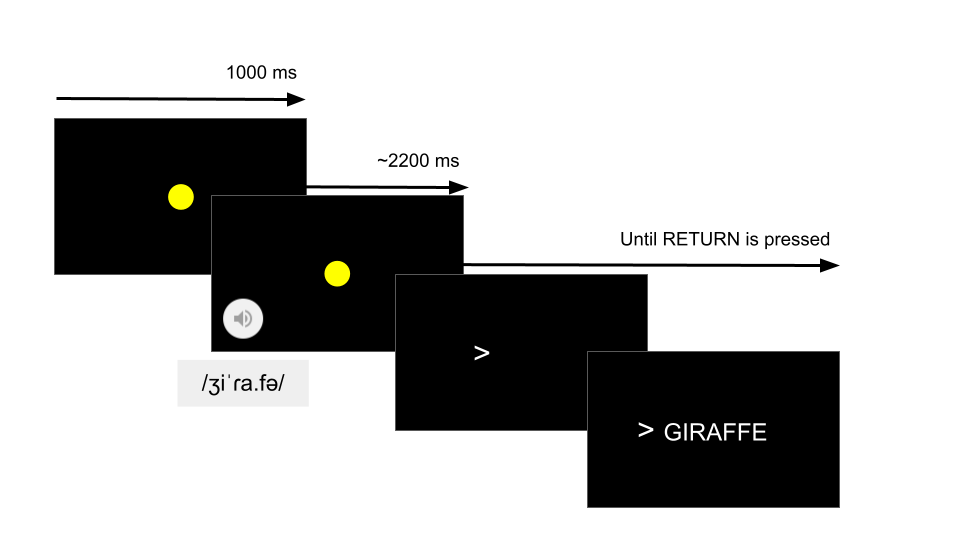
\includegraphics[keepaspectratio]{_assets/img/design.png}}

}

\end{figure}%

\subsubsection{Data analysis}\label{data-analysis}

\paragraph{Data processing.}\label{data-processing}

After data collection, participants' answers were manually coded into
the following categories: \emph{Correct}, \emph{Typo}, \emph{Wrong},
\emph{False friend}, \emph{Other}. A response was coded as
\emph{Correct} if the provided string of characters was identical to the
orthographic form of the correct translation. A response was coded as
\emph{Typo} if the participant provided a string of characters that was
only one edit distance (addition, deletion, or substitution) apart from
the orthographic form of the correct translation (e.g., ``pengiun''
instead of ``penguin''), as long as the response did not correspond to a
distinct English word. A response was coded as \emph{False friend} if
the participant's response was incorrect, but phonologically similar to
the presented word. Responses not meeting the criteria for previous
categories were labelled as \emph{Wrong} or \emph{Other} (see Data
analysis section for more details). Both \emph{Correct} and \emph{Typo}
responses were considered as correct, while \emph{Wrong} and \emph{False
friend} responses were considered as incorrect. \emph{Other} responses
were excluded from data analysis. Trials in which participants took
longer than 10 seconds to respond were also excluded. Participants
contributed a total of 5,206 valid trials (2,604 in Catalan, 2,602 in
Spanish). The task took approximately 15 minutes to complete.

\paragraph{Modelling approach and statistical
inference.}\label{modelling-approach-and-statistical-inference}

We modelled the probability of participants guessing the correct
translation of each presented word using a generalised multilevel
Bayesian regression model with a Bernoulli logit link distribution. We
included as fixed effects the intercept, the main effects of
\emph{Frequency}, \emph{Similarity}, \emph{CLPN}, and \emph{Group}
(sum-coded as \texttt{cat-ENG\ =\ -0}, \texttt{spa-ENG\ =\ +0.5},
\citeproc{ref-schad2020capitalize}{Schad et al., 2020}) and the
three-way interaction between \emph{Similarity}, \emph{CLPN}, and
\emph{Group}. The predictor \emph{Group} was included to account for any
differences in task performance between English participants translating
Catalan and Spanish words. We also included participant-level random
intercepts and slopes for the main effects and the interaction. Eq. 1
shows a formal description of the model.

\begin{equation}\phantomsection\label{eq-1}{
\begin{aligned}
&\textbf{Likelihood}  \\
y_{i} \sim & \text{Bernoulli}(p_{i}) \\ \\
&\textbf{Parameters}  \\
\text{Logit}(p_{i}) = &  \beta_{0[p,w]} + \beta_{1[p]} \text{Frequency}_{i} + \beta_{2[p]} \text{Similarity}_i +  \beta_{3[p]} \text{CLPN}_i + \beta_{4[p]} \text{Group}_i + \\
&\beta_{5[p]} (\text{Similarity}_i \times \text{CLPN}_i) + \beta_{6[p]} (\text{Similarity}_i \times \text{Group}_i) + \\
& \beta_{7[p]} (\text{CLPN}_i \times \text{Group}_i) + \beta_{8[p]} (\text{Similarity}_i \times \text{CLPN}_i \times \text{Group}_i) \\ \\
\beta_{0-8[p,w]} \sim & \mathcal{N}(\mu_{\beta_{j}}, \sigma_{\beta_{j}}) \text{, for participant } p \text{ in 1, ..., } P \text{ and  word } w \text{ in 1, ..., } W \\
\beta_{1-8[p]} \sim &  \mathcal{N}(\mu_{\beta_{j}}, \sigma_{\beta_{j}}) \text{, for participant } p \text{ in 1, ..., } P \\ \\
&\textbf{Prior}  \\
\mu_{\beta_{p,w}}  \sim &  \mathcal{N}(0, 0.1) \\
\sigma_{\beta_{p}},  \sigma_{\beta_{w}} \sim & \text{HalfCauchy}(0, 0.1) \\
\rho_{p}, \rho_{w} \sim & \text{LKJCorr}(8) \\
\end{aligned}
}\end{equation}

We followed Kruschke and Liddell
(\citeproc{ref-kruschke2018bayesian}{2018})'s guidelines for statistical
inference. We first specified a region of practical equivalence (ROPE)
around zero ({[}-0.1, +0.1{]}, in the logit scale). This area indicates
the values of the regression coefficients that we considered equivalent
to zero. We then computed the 95\% posterior credible intervals (CrI) of
the regression coefficients of interest, which indicates the most likely
range of values that contains the true value of the coefficient with
95\% probability. Finally, for each regression coefficient we calculated
the proportion of the 95\% CrI that fell inside the ROPE, noted as
\emph{p}(ROPE). This proportion indicates the probability that the true
value of the coefficient is equivalent to zero. For instance, if the
\emph{p}(ROPE) of a regression coefficient \(\beta\) is 0.5, this
indicates that there is a 50\% probability that the true value of
\(\beta\) is zero or equivalent to zero, given the data. If
\emph{p}(ROPE)=0.01, this indicates that there is a 1\% probability that
the true value of the regression coefficient is zero or equivalent. If
\emph{p}(ROPE)=0.99, this indicates that there is a 99\% probability
that the true value of the regression coefficient is zero or equivalent.

All analyses were performed in the R environment
(\citeproc{ref-rcoreteam2013language}{R Core Team, 2013}). We used the
tidyverse family of R packages
(\citeproc{ref-wickham2019welcome}{Wickham et al., 2019}) to process
data and to generate figures. We used the \texttt{brms} R package
(\citeproc{ref-burkner2017brms}{Bürkner, 2017}) using the
\texttt{cmdstanr} back-end to the Stan probabilistic language
(\citeproc{ref-carpenter2017stan}{Carpenter et al., 2017}) to estimate
and compare the models (see \#apx-diagnostics for model diagnostics).
Numeric predictors were standardised before entering the model by
subtracting the mean and dividing by the standard deviation.

\subsection{Results}\label{results}

We collected data for a total of 6,446 trials completed by 72
participants. We excluded trials in which participants did not enter any
text (\emph{n} = 72), in which a response in a language other than
English was provided (e.g., ``\texttt{agua}'', \emph{n} = 51), in which
participants did not provide a whole word (e.g., ``\texttt{f}'',
\emph{n} = 5), and in which participants added comments to the
experimenter (e.g., ``\texttt{unsure}'', \emph{n} = 13). In addition, we
excluded data from participants that self-rated their oral and/or
written skills in Catalan and Spanish, or any other second language as
four or higher in a five-point scale (\emph{n} = 2), were diagnosed with
a language disorder (\emph{n} = 1), or did not contribute more than 80\%
of valid trials (\emph{n} = 9).

After applying trial-level and participant-level exclusion criteria, the
resulting dataset included 5,204 trials provided by 54 participants. Of
those trials, 2,602 were provided by 27 participants who listened to
Catalan words, and 2,604 trials were provided by 32 participants who
listened to Spanish words. Responses given by English participants to
Catalan presented words were 5.35 characters long on average
(\emph{Median} = 5, \emph{SD} = 1.79, Range = 1-14), while their
translations to Spanish responses were 5.57 characters long on average
(\emph{Median} = 5, \emph{SD} = 1.97, Range = 2-21).

Table~\ref{tbl-dataset} shows a summary of participants' accuracy across
Experiments 1, 2, and 3. Participants translating Catalan words and
participants translating Spanish words performed equivalently, as
indicated by the regression coefficient of \emph{Group} (\(\beta\) =
-0.165, 95\% CrI = {[}-0.482, 0.125{]}, \emph{p}(ROPE) = 0.302).
Overall, participants responded less accurately to words with more CLPNs
than to words with fewer CLPNs, regardless of the amount of phonological
similarity between the presented word and its translation. This is
indicated by the size of the regression coefficient of the two-way
interaction between \emph{Similarity} and \emph{CLPN} (\(\beta\) =
-0.236, 95\% CrI = {[}-0.362, -0.118{]}, \emph{p}(ROPE) = 0.015). As
anticipated, participants' performance benefited from an increase in
\emph{Similarity} (\(\beta\) = 1.437, 95\% CrI = {[}1.314, 1.544{]},
\emph{p}(ROPE) = 0), while the number of \emph{CLPN} had the opposite
effect (\(\beta\) = -0.167, 95\% CrI = {[}-0.352, -0.01{]},
\emph{p}(ROPE) = 0.2). Figure~\ref{fig-epreds-1} illustrates the
posterior of the average predictions of the model for words with
different values of \emph{Similarity} and \emph{CLPN}.

\begin{table}

{\caption{{Summary of participants' accuracy in the translation
elicitation task across Experiments 1, 2, and 3.}{\label{tbl-dataset}}}
\vspace{-20pt}}

\begin{longtable*}{l|rrrrrrrrr}
\toprule
\multicolumn{1}{l}{} &  & \multicolumn{4}{c}{Accuracy (\%)} & \multicolumn{4}{c}{Valid trials} \\ 
\cmidrule(lr){3-6} \cmidrule(lr){7-10}
\multicolumn{1}{l}{} & N & Mean & SD & SE & Range & Mean & N trials & SD & Range \\ 
\midrule\addlinespace[2.5pt]
\multicolumn{10}{l}{Experiment 1} \\ 
\midrule\addlinespace[2.5pt]
spa-ENG & $27$ & $15.86$ & $5.20$ & $3.05$ & $8.82$–$28.71$ & $96.37$ & $2,602$ & $2.88$ & $87$–$98$ \\ 
cat-ENG & $32$ & $18.48$ & $4.89$ & $3.27$ & $10.84$–$32.56$ & $81.38$ & $2,604$ & $3.17$ & $71$–$83$ \\ 
\midrule\addlinespace[2.5pt]
\multicolumn{10}{l}{Experiment 2} \\ 
\midrule\addlinespace[2.5pt]
cat-SPA & $21$ & $48.30$ & $5.29$ & $10.54$ & $38.27$–$58.97$ & $79.14$ & $1,662$ & $3.14$ & $72$–$82$ \\ 
\midrule\addlinespace[2.5pt]
\multicolumn{10}{l}{Experiment 3} \\ 
\midrule\addlinespace[2.5pt]
spa-ENG & $31$ & $20.92$ & $8.29$ & $3.76$ & $5.88$–$44.12$ & $97.45$ & $3,021$ & $1.80$ & $88$–$98$ \\ 
cat-ENG & $32$ & $19.74$ & $4.94$ & $3.49$ & $10.34$–$27.91$ & $82.75$ & $2,648$ & $0.44$ & $82$–$83$ \\ 
\bottomrule
\end{longtable*}

\end{table}

\begin{figure}

\caption{\label{fig-epreds-1}Posterior model-predicted mean accuracy in
Experiment 1. Predictions were generated from 4,000 posterior samples,
extracted for different values of \emph{CLPN} (0, 2, 4, 8, 12) and
\emph{Similarity} (1-100). Predictions are plotted separately for
English participants translating Catalan words, and for English
participants translating Spanish words. Lines indicate mean predictions,
and intervals indicate 95\%, 89\%, 78\%, 67\%, and 50\% credible
intervals (CrI).}

\centering{

\pandocbounded{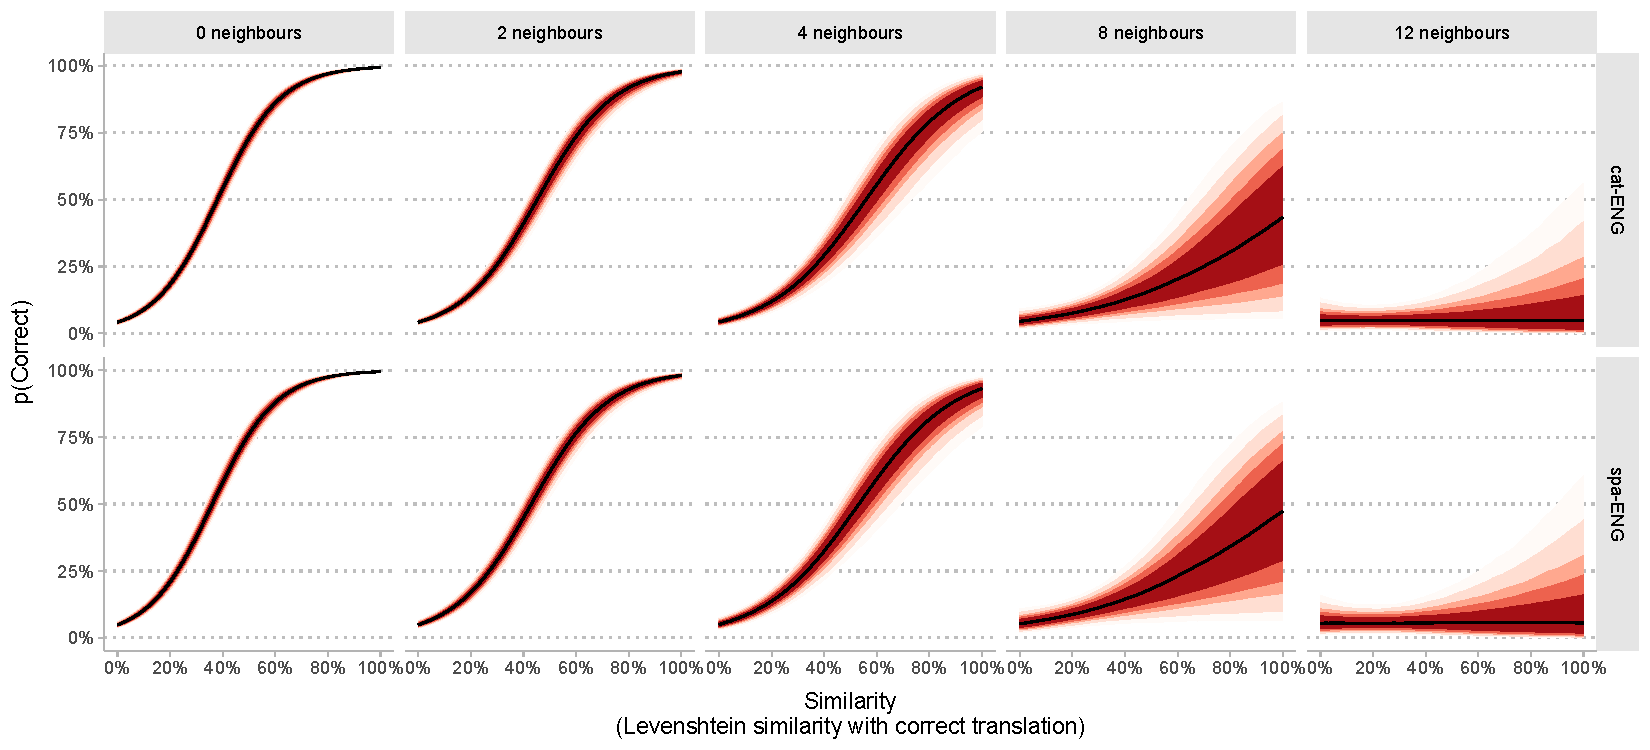
\includegraphics[keepaspectratio]{manuscript_files/figure-pdf/fig-epreds-1-1.pdf}}

}

\end{figure}%

\subsection{Discussion}\label{discussion}

In Experiment 1, we investigated the extent to which the phonological
similarity between translation equivalents is sufficient for successful
word translation, in the absence of conceptual knowledge about the
presented word. We tested two groups of monolingual British
English-native adults in a translation task that involved words in
Catalan or Spanish, two languages participants reported having no prior
familiarity with. Participants benefited strongly from phonological
similarity when the correct translation of the presented words in
Catalan or Spanish had few English phonological neighbours with higher
lexical frequency. As the number of higher-frequency English
phonological neighbours increased, both participants' accuracy and the
impact of phonological similarity approached zero. This suggests that
word-forms in an unfamiliar language have a strong potential to activate
their translation equivalents in the native language, provided some
phonological similarity between both words, and the absence of more
frequent phonological neighbors.

Participants in Experiment 1 were surprisingly good at translating words
from Catalan and Spanish (two unfamiliar languages) to their native
language. If English participants were likely to activate the correct
English translations of the presented words in Catalan and Spanish, it
is possible that speakers of typologically closer languages to Catalan
and Spanish may benefit even more strongly from phonological similarity
in the same task. English is a Germanic language (like Dutch or German),
while Catalan and Spanish are Romance languages (like Italian, French,
Portuguese). English shares fewer phonologically similar translations
with Romance languages than Romance languages share with each other. It
is possible that the probability of homophonic translations is higher
when listening to an unfamiliar language from the same typological
family as the native language. We tested this hypothesis in Experiment
2.

\section{Experiment 2}\label{experiment-2}

Results in Experiment 1 suggest that English natives were able to
exploit the phonological similarity between unfamiliar words in Catalan
and Spanish to provide accurate translations to English. English, a
Germanic language, is relatively distant from Catalan and Spanish, two
Romance languages. In comparison, Catalan and Spanish are typologically
close languages that share many more cognates. In Experiment 2, we
investigated whether listeners of an unfamiliar but typologically closer
language benefit more strongly from phonological similarity when
performing the same task as in Experiment 1. To this aim, we presented
Spanish participants, who reported little-to-no prior familiarity with
Catalan, with Catalan words.

\subsection{Methods}\label{methods-1}

We collected data from 33 Spanish native adults living in Spain
(\emph{Mean} = 21.85 years, \emph{SD} = 3, Range = 18-33, 28, 5 female).
Data collection took place from June 8th, 2020 to June 28th, 2020.
Participants in Spain were contacted via announcements at the University
campus(es), and were compensated €5 or an Amazon voucher for the same
value. Participants gave informed consent before providing any data and
the study was conducted in accordance with ethical standards of the
Declaration of Helsinki and the protocol was approved by the Drug
Research Ethical Committee (CEIm) of the IMIM Parc de Salut Mar
(2020/9080/I).

Stimuli were the same list of Catalan stimuli as in Experiment 1.
Procedure and data analysis were identical as in Experiment 1, with the
only exception that the statistical model did not include the
\emph{Group} predictor, given that only one group (\texttt{cat-SPA})
participated in this experiment.

\subsection{Results}\label{results-1}

We collected data for a total of 5,412 trials completed by 33
participants. We excluded trials in which participants did not enter any
text (\emph{n} = 44), in which a response in a language other than
Spanish was provided (\emph{n} = 51), in which participants did not
provide a whole word (\emph{n} = 7), and in which participants added
comments to the experimenter (\emph{n} = 1). In addition, we excluded
data from participants that self-rated their oral and/or written skills
in Catalan or any other second language as four or higher in a
five-point scale (\emph{n} = 22), were diagnosed with a developmental
language disorder (\emph{n} = 1), or did not contribute more than 80\%
of valid trials (\emph{n} = 9). After applying trial-level and
participant-level inclusion criteria, the resulting dataset included
1,662 trials provided by 42 participants. Responses given by
participants were 5.6 characters long on average (\emph{Median} = 5,
\emph{SD} = 1.6, Range = 2-12).

Overall, participants responded less accurately to words with more CLPNs
than to words with fewer CLPNs, regardless of the amount of phonological
similarity between the presented word and its translation. This is
indicated by the size of the regression coefficient of the two-way
interaction between \emph{Similarity} and \emph{CLPN} (\(\beta\) =
-0.162, 95\% CrI = {[}-0.369, 0.032{]}, \emph{p}(ROPE) = 0.268). As
anticipated, participants' performance benefited from an increase in
\emph{Similarity} (\(\beta\) = 1.906, 95\% CrI = {[}1.712, 2.086{]},
\emph{p}(ROPE) = 0), while the number of \emph{CLPN} had the opposite
effect (\(\beta\) = -0.274, 95\% CrI = {[}-0.613, 0.088{]},
\emph{p}(ROPE) = 0.14). Figure~\ref{fig-epreds-2} illustrates the
posterior of the average predictions of the model for words with
different values of \emph{Similarity} and \emph{CLPN}.

\begin{figure}

\caption{\label{fig-epreds-2}Posterior model-predicted mean accuracy in
Experiment 1. Predictions were generated from 4,000 posterior samples,
extracted for different values of \emph{CLPN} (0, 2, 4, 8, 12) and
\emph{Similarity} (1-100). Lines indicate mean predictions, and
intervals indicate 95\%, 89\%, 78\%, 67\%, and 50\% credible intervals
(CrI).}

\centering{

\pandocbounded{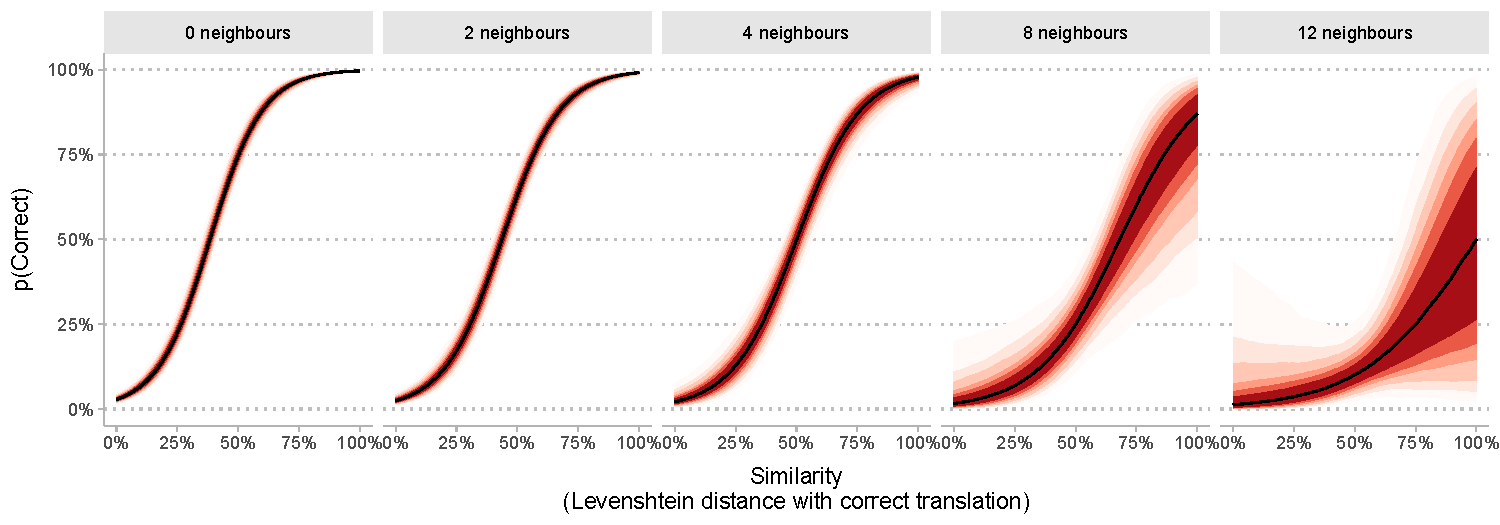
\includegraphics[keepaspectratio]{manuscript_files/figure-pdf/fig-epreds-2-1.pdf}}

}

\end{figure}%

In order to compare the results from Experiments 1 and 2 directly, we
fit a model on the joint datasets from both experiments. This model
included all predictors from the models presented in Experiments 1 and
2, and the predictor \emph{Experiment} with levels
\texttt{"Experiment\ 1"} and \texttt{"Experiment\ 2"}, and a three-way
interaction between \emph{Experiment}, \emph{Similarity}, and
\emph{CLPN}. The \emph{Experiment} variable was sum-coded as
\texttt{-0.5\ =\ Experiment\ 1} and \texttt{+0.5\ =\ Experiment\ 2}. All
two-way interactions between the three predictors were also included.
The effect of \emph{CLPN} on \emph{Similarity} was equivalent in both
groups, as indicated by the coefficient of the three-way way interaction
(\(\beta\) = 0.105, 95\% CrI = {[}-0.151, -0.043{]}). The posterior
probability of this coefficient being equivalent to
zero---\emph{p}(ROPE)---was 0.422), that is, inconclusive. The
coefficient of the interaction term between \emph{Experiment} and
\emph{CLPN} was also equivalent to zero (\(\beta\) = -0.09, 95\% CrI =
{[}-0.458, 0.346{]}, \emph{p}(ROPE) = 0.361), suggesting that
participants from Experiments 1 and 2 were affected by CLPN on a similar
basis. Finally, the coefficient of the interaction between
\emph{Experiment} and \emph{Similarity} was different from zero
(\(\beta\) = -0.09, 95\% CrI = {[}0.326, 0.785{]}, \emph{p}(ROPE) = 0),
with a positive sign indicating that the increments in \emph{Similarity}
were associated with a larger increment in probability of correct
translation in Experiment 2, compared to in Experiment 1: for an average
value of \emph{CLPN}, participants in Experiment 2 benefited more
strongly from \emph{Similarity} than participants in Experiment 1.

\subsection{Discussion}\label{discussion-1}

Experiment 2 was an extension of Experiment 1 to a population of
monolinguals whose native language is typologically close to the
presented language. We presented Catalan words to Spanish native adults
who were reportedly unfamiliar with Catalan. Our results indicate a
similar pattern of results as those in Experiment 1: participants were
able to provide correct translations of presented Catalan words,
provided that the Catalan words shared some degree of phonological
similarity with their Spanish translation, and that the number of
phonological neighbours with higher lexical frequency was reduced. In
contrast with the results in Experiment 1, the positive impact of
phonological similarity on participants' performance in Experiment 2
larger. Spanish natives in Experiment 2 exploited phonological
similarity more strongly than English natives in Experiment 1. Overall,
this suggests that participants in Experiment 2, who were natives of a
typologically similar language (Spanish) to the presented language
(Catalan), benefited more strongly from phonological similarity than
participants in Experiment 1, who were natives of a typologically less
similar language (English) to the presented language (Catalan, Spanish).
Participants from both Experiment 1 and 2 benefited strongly from
phonological similarity to correctly translate words from a non-native,
reportedly unfamiliar language. This pattern of results holds for most
of the presented stimuli, but some low-similarity Catalan and Spanish
words were responded to surprisingly accurately by English listeners.
Given that participants were reportedly unfamiliar with both languages,
it was expected that participants would be very unlikely to provide
correct translations for words sharing little to no phonological
similarity to their correct translation. Table~\ref{tbl-surprises} shows
a list of Catalan and Spanish words to which participants provided
responses with \(\geq\) 10 average accuracy.

\begin{table}

{\caption{{List of items with unexpectedly high accuracy: the
Levenshtein similarity score between the presented word (in Catalan or
Spanish) and their correct English translation is zero, but
participants, who are reportedly unfamiliar with the presented language,
were on average \textgreater10\% likely to guess the correct
translation.}{\label{tbl-surprises}}}
\vspace{-20pt}}

\centering
\begin{tblr}[         %% tabularray outer open
]                     %% tabularray outer close
{                     %% tabularray inner open
colspec={Q[]Q[]Q[]Q[]},
cell{2}{1}={c=4}{},cell{8}{1}={c=4}{},cell{25}{1}={c=4}{},
cell{3}{1}={preto={\hspace{1em}}},
cell{4}{1}={preto={\hspace{1em}}},
cell{5}{1}={preto={\hspace{1em}}},
cell{6}{1}={preto={\hspace{1em}}},
cell{7}{1}={preto={\hspace{1em}}},
cell{9}{1}={preto={\hspace{1em}}},
cell{10}{1}={preto={\hspace{1em}}},
cell{11}{1}={preto={\hspace{1em}}},
cell{12}{1}={preto={\hspace{1em}}},
cell{13}{1}={preto={\hspace{1em}}},
cell{14}{1}={preto={\hspace{1em}}},
cell{15}{1}={preto={\hspace{1em}}},
cell{16}{1}={preto={\hspace{1em}}},
cell{17}{1}={preto={\hspace{1em}}},
cell{18}{1}={preto={\hspace{1em}}},
cell{19}{1}={preto={\hspace{1em}}},
cell{20}{1}={preto={\hspace{1em}}},
cell{21}{1}={preto={\hspace{1em}}},
cell{22}{1}={preto={\hspace{1em}}},
cell{23}{1}={preto={\hspace{1em}}},
cell{24}{1}={preto={\hspace{1em}}},
cell{26}{1}={preto={\hspace{1em}}},
cell{27}{1}={preto={\hspace{1em}}},
cell{28}{1}={preto={\hspace{1em}}},
cell{29}{1}={preto={\hspace{1em}}},
cell{30}{1}={preto={\hspace{1em}}},
cell{31}{1}={preto={\hspace{1em}}},
row{1}={,cmd=\bfseries,},
hline{1,2}={1,2,3,4}{solid, 0.1em, black},
row{2}={,cmd=\bfseries,},
hline{3}={1,2,3,4}{solid, 0.1em, black},
row{8}={,cmd=\bfseries,},
hline{8,9}={1,2,3,4}{solid, 0.1em, black},
row{25}={,cmd=\bfseries,},
hline{25,26}={1,2,3,4}{solid, 0.1em, black},
}                     %% tabularray inner close
\toprule
Translation & IPA & Accuracy (\%) & SE \\ \midrule %% TinyTableHeader
Experiment 1 (cat-ENG) &&& \\
cavall - horse       & \textipa{/k@'ba}\textlambda\textipa{/ - /hO:s/}                                  & 17.14 & 6.37 \\
llibre - book        & \textipa{/"}\textlambda\textipa{i.BR@/ - /bUk/}                                  & 17.14 & 6.37 \\
camisa - shirt       & \textipa{/ka.'mi.za/ - /S3:t/}                                                     & 16.67 & 6.21 \\
poma - apple         & \textipa{/"po.ma/ - /"aepl/}                                                       & 16.67 & 6.21 \\
cama - leg           & \textipa{/"ka.m@/ - /lEg/}                                                         & 11.11 & 5.24 \\
Experiment 2 (spa-ENG) &&& \\
pantalon - trousers  & \textipa{/paN.ta"lon/ - /"traUz@z/}                                                & 77.42 & 7.51 \\
naranja - orange     & \textipa{/na"RaN.xa/ - /"6rIn}\textdyoghlig\textipa{/}                           & 41.94 & 8.86 \\
leche - milk         & \textipa{/"le.}\textteshlig\textipa{e/ - /mIlk/}                                 & 35.48 & 8.59 \\
toro - bull          & \textipa{/"to.Ro/ - /bUl/}                                                         & 33.33 & 8.61 \\
libro - book         & \textipa{/"li.BRo/ - /bUk/}                                                        & 30.00 & 8.37 \\
cebra - zebra        & \textipa{/"Te.bRa/ - /"zi:br@/}                                                    & 29.03 & 8.15 \\
pan - bread          & \textipa{/pan/ - /brEd/}                                                           & 29.03 & 8.15 \\
pollo - chicken      & \textipa{/"po.}\textlambda\textipa{o/ - /"}\textteshlig\textipa{IkIn/}         & 26.67 & 8.07 \\
jirafa - giraffe     & \textipa{/xi'Ra.fa/ - /}\textdyoghlig\textipa{I"rA:f/}                           & 20.69 & 7.52 \\
perro - dog          & \textipa{/pe.ro/ - /d6g/}                                                          & 16.13 & 6.61 \\
pluma - feather      & \textipa{/plu.ma/ - /"fED@/}                                                       & 16.13 & 6.61 \\
puerta - door        & \textipa{/pwer.ta/ - /dO:/}                                                        & 16.13 & 6.61 \\
pie - foot           & \textipa{/pje/ - /fUt/}                                                            & 12.90 & 6.02 \\
caballo - horse      & \textipa{/ka"Ba.}\textlambda\textipa{o/ - /hO:s/}                                & 10.34 & 5.66 \\
bocadillo - sandwich & \textipa{/bo.ka"di.}\textlambda\textipa{o/ - /"saenwI}\textdyoghlig\textipa{/} & 10.00 & 5.48 \\
globo - balloon      & \textipa{/"glo.Bo/ - /b@"lu:n/}                                                    & 10.00 & 5.48 \\
Experiment 3 (cat-SPA) &&& \\
fulla - hoja         & \textipa{/"fu.}\textlambda\textipa{@/ - /"o.xa/}                                 & 30.43 & 9.59 \\
ull - ojo            & \textipa{/u}\textlambda\textipa{/ - /"o.xo/}                                     & 21.74 & 8.60 \\
got - vaso           & \textipa{/"gOt/ - /"ba.so/}                                                        & 20.00 & 8.00 \\
entrepa - bocadillo  & \textipa{/ˌen.tR@"pa/ - /bo.ka"di.}\textlambda\textipa{o/}                       & 13.04 & 7.02 \\
mirall - espejo      & \textipa{/mi"Ra}\textlambda\textipa{/ - /es'pe.xo/}                              & 12.50 & 6.75 \\
\bottomrule
\end{tblr}

\end{table}

It is likely that participants had prior knowledge of these words
despite having reported little to no familiarity with the presented
language (Catalan or Spanish). One possibility is that participants had
previously encountered these words embedded in English linguistic input.
Spanish words percolate English speech with relative frequency, via
different sources such as popular culture, songs, TV programs, etc. In
addition, words from languages other than Spanish or Catalan, but with
high similarity to the Spanish or Catalan words (e.g., cognates from
Italian or French) might appear in English speech as well. Such prior
knowledge might not be specific to the low-similarity words highlighted
before. Participants may also have had prior knowledge about
higher-similarity words, which could have contributed to participants
responding to such words more accurately than without such prior
knowledge. In the case of higher-similarity words, it is more difficult
to disentangle the extent to which participants' accuracy is a function
of pure phonological similarity, or prior knowledge they had about the
meaning of Spanish words. Experiment 3 was addressed at investigating
the issue of prior knowledge.

\section{Experiment 3}\label{experiment-3}

Experiment 3 is a replication of Experiment 1, in which we collected
additional data about participants' prior familiarity with the presented
Catalan and Spanish words, in addition to the same translation task
presented to participants in Experiment 1.

\subsection{Methods}\label{methods-2}

We collected data from 64 British English native adults living in United
Kingdom (\emph{Mean} = 22.02 years, \emph{SD} = 2.49, Range = 18-26, 36,
28 female). Data collection took place from October 22th, 2022 to
October 23th, 2022. Participants were recruited via Prolific (5£
compensation) and SONA (compensation in academic credits), and gave
informed consent before providing any data and the study was conducted
in accordance with ethical standards of the Declaration of Helsinki and
the protocol was approved by the University of Oxford Medical Sciences
Inter-Divisional Research Ethics Committee (IDREC) (R60939/RE007).
Participants were asked to complete the experiment using a laptop in a
quiet place with good internet connection. Stimuli were the same lists
of Catalan and Spanish stimuli as in Experiment 1.

The experiment was implemented online using Qualtrics (Qualtrics, Provo,
UT). This platform was chosen to allow easier presentation of survey
questions aimed to probe prior understanding of the presented words and
participants' confidence ratings of their answers. With the exception of
these additional questions, we attempted to replicate the procedure of
Experiment 1 as closely as possible. The Spanish and Catalan audio
stimuli used were identical the materials in Experiment 1. Participants
were randomly assigned to the Catalan or Spanish lists. The Catalan list
had 83 trials and the Spanish list had 99 trials. Participants first
completed the consent form followed by the questionnaire about
demographic status, language background and set up. They then proceeded
to the experimental task.

In each trial, participants listened to the audio stimulus by clicking
on the \texttt{PLAY} button. For comparability to the PsychoPy version,
participants were only allowed to play the audio one time. Participants
were explicitly told that they would be only allowed to listen once. The
\texttt{PLAY} button vanished after one playthrough. Participants then
had to answer three questions based on the audio they had heard on that
trial. These questions were presented on the same page, directly below
the audio player. They were first asked whether they knew the presented
word (multiple choice---\emph{yes}/\emph{no}). Regardless of their
answer on the first question, participants were asked what they thought
the translation of the word was in English (or their best guess), and
instructed to type their answer in the provided text box. Finally, they
were asked to rate how confident they were in their answer on a scale of
0 to 7, where 7 was ``very confident'' and 0 was ``not confident''.
There was no time limit on the response phase. All questions had to be
answered to proceed to the next trial.

Participants first completed 5 practice trials with English words as the
audio stimulus (ambulance, cucumber, elephant, pear, turtle). The words
were recorded by a female native speaker of British English. These
trials acted as attention checks, as participants should always answer
``yes'' to the first question on prior word knowledge and be able to
accurately transcribe the word they heard. Following the practice phase,
participants completed the test phase where they heard either Spanish
words or Catalan words.

\subsection{Results}\label{results-2}

We collected data for a total of 6,016 trials completed by 64
participants. We excluded trials in which participants did not enter any
text (\emph{n} = 0), provided a response in a language other than
English (\emph{n} = 9), did not provide a whole word (\emph{n} = 0), or
added comments to the experimenter (\emph{n} = 0). In addition, we
excluded data from participants that self-rated their oral and/or
written skills in Catalan and Spanish, or any other second language as
four or higher in a five-point scale (\emph{n} = 2), were diagnosed with
a language disorder (\emph{n} = 0), or did not contribute more than 80\%
of valid trials (\emph{n} = 1).

After applying trial-level and participant-level inclusion criteria, the
resulting dataset included 5,888 trials provided by 63 participants. Of
those trials, 3,145 were provided by 31 participants who listened to
Catalan words, and 2,743 trials were provided by 32 participants who
listened to Spanish words.

From the 3,145 total responses provided by English participants who
listened to Catalan words, participants reported having prior knowledge
of the presented Catalan words in 446 (14.18\%) of them. In those
responses, participants reported an average of 5.05 confidence in the
0-8 scale (\emph{SD} = 1.94). For responses where no prior knowledge of
the presented word was reported, average confidence was 1.13 (\emph{SD}
= 1.38). From the 2,743 total responses provided by English participants
who listened to Spanish words, participants reported having prior
knowledge of the presented Spanish words in 197 (7.18\%) of them. In
those responses, participants reported an average of 4.79 confidence in
the 0-8 scale (\emph{SD} = 1.82). For responses where no prior knowledge
of the presented word was reported, average confidence was 1.25
(\emph{SD} = 1.66). Before data analysis, responses where participants
reported prior knowledge about the meaning of the presented Catalan or
Spanish word were excluded from the dataset.

Responses given by English participants to Catalan presented words were
5.49 characters long on average (\emph{Median} = 5, \emph{SD} = 1.71,
Range = 1-14), while their translations to Spanish responses were 5.39
characters long on average (\emph{Median} = 5, \emph{SD} = 1.75, Range =
1-20).

Overall, participants reported prior knowledge more often for the
Spanish words that showed unexpectedly high accuracy in Experiment 1
(see Discussion in Experiment 2) than for words with expected accuracy
(see Figure~\ref{fig-knowledge}). Participants reported prior knowledge
of Catalan words with unexpected accuracy in Experiment 1 as often as
those with expected accuracy. This suggests that participants in
Experiment 1 may have relied, to some extent, on their prior knowledge
about form-meaning mappings to correctly translate some Spanish words.
To isolate such an effect of prior Spanish knowledge, we ran the same
analysis as in Experiment 1 on the newly collected translations from
Experiment 3, now excluding responses to words for which participants
reported prior knowledge.

\begin{figure}

\caption{\label{fig-knowledge}Catalan and Spanish prior word knowledge
reported by English native participants in Experiment 3. The X-axis
indicates the proportion of participants that reported prior knowledge
with the word. The Y-axis indicates participants' accuracy (the
proportion of participants that translated the word correctly). For
visualisation purposes, data points have been aggregated so that numbers
and color coding show the number of data points with identical accuracy
and proportion of reported knowledge.}

\centering{

\pandocbounded{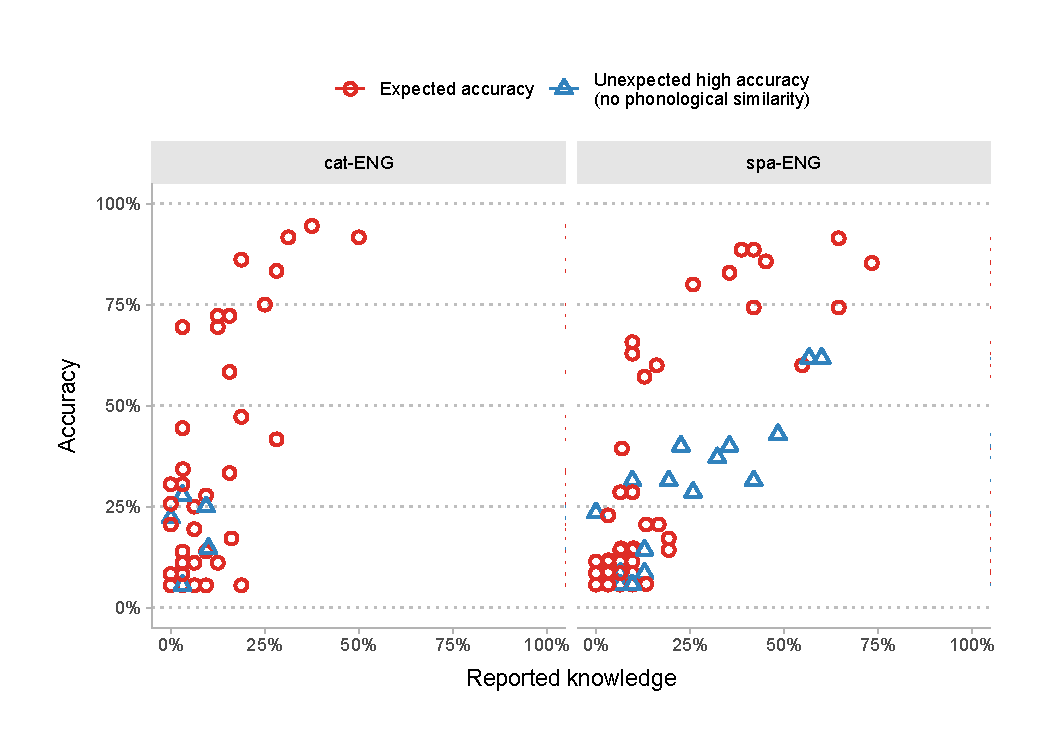
\includegraphics[keepaspectratio]{manuscript_files/figure-pdf/fig-knowledge-1.pdf}}

}

\end{figure}%

Participants translating Catalan words and participants translating
Spanish words performed similarly, as indicated by the regression
coefficient of \emph{Group} (\(\beta\) = -0.065, 95\% CrI = {[}-0.389,
-0.118{]}, \emph{p}(ROPE) = 0.422). Overall, both groups of participants
responded less accurately to words with more CLPNs than to words with
fewer CLPNs, regardless of the amount of phonological similarity between
the presented word and its translation. This is indicated by the size of
the regression coefficient of the two-way interaction between
\emph{Similarity} and \emph{CLPN} (\(\beta\) = -0.252, 95\% CrI =
{[}-0.385, -0.118{]}, \emph{p}(ROPE) = 0.015). As anticipated,
participants' performance benefited from an increase in
\emph{Similarity} (\(\beta\) = 1.532, 95\% CrI = {[}1.41, 1.657{]},
\emph{p}(ROPE) = 0), while the number of \emph{CLPN} had the opposite
effect (\(\beta\) = -0.288, 95\% CrI = {[}-0.523, -0.082{]},
\emph{p}(ROPE) = 0.023). Figure~\ref{fig-epreds-3} illustrates the
posterior of the average predictions of the model for words with
different values of \emph{Similarity} and \emph{CLPN}.

\begin{figure}

\caption{\label{fig-epreds-3}Posterior model-predicted mean accuracy in
Experiment 3. Predictions were generated from 4,000 posterior samples,
extracted for different values of \emph{CLPN} (0, 2, 4, 8, 12) and
\emph{Similarity} (1-100). Predictions are plotted separately for
English participants translating Catalan words, and for English
participants translating Spanish words. Lines indicate mean predictions,
and intervals indicate 95\%, 89\%, 78\%, 67\%, and 50\% credible
intervals (CrI).}

\centering{

\pandocbounded{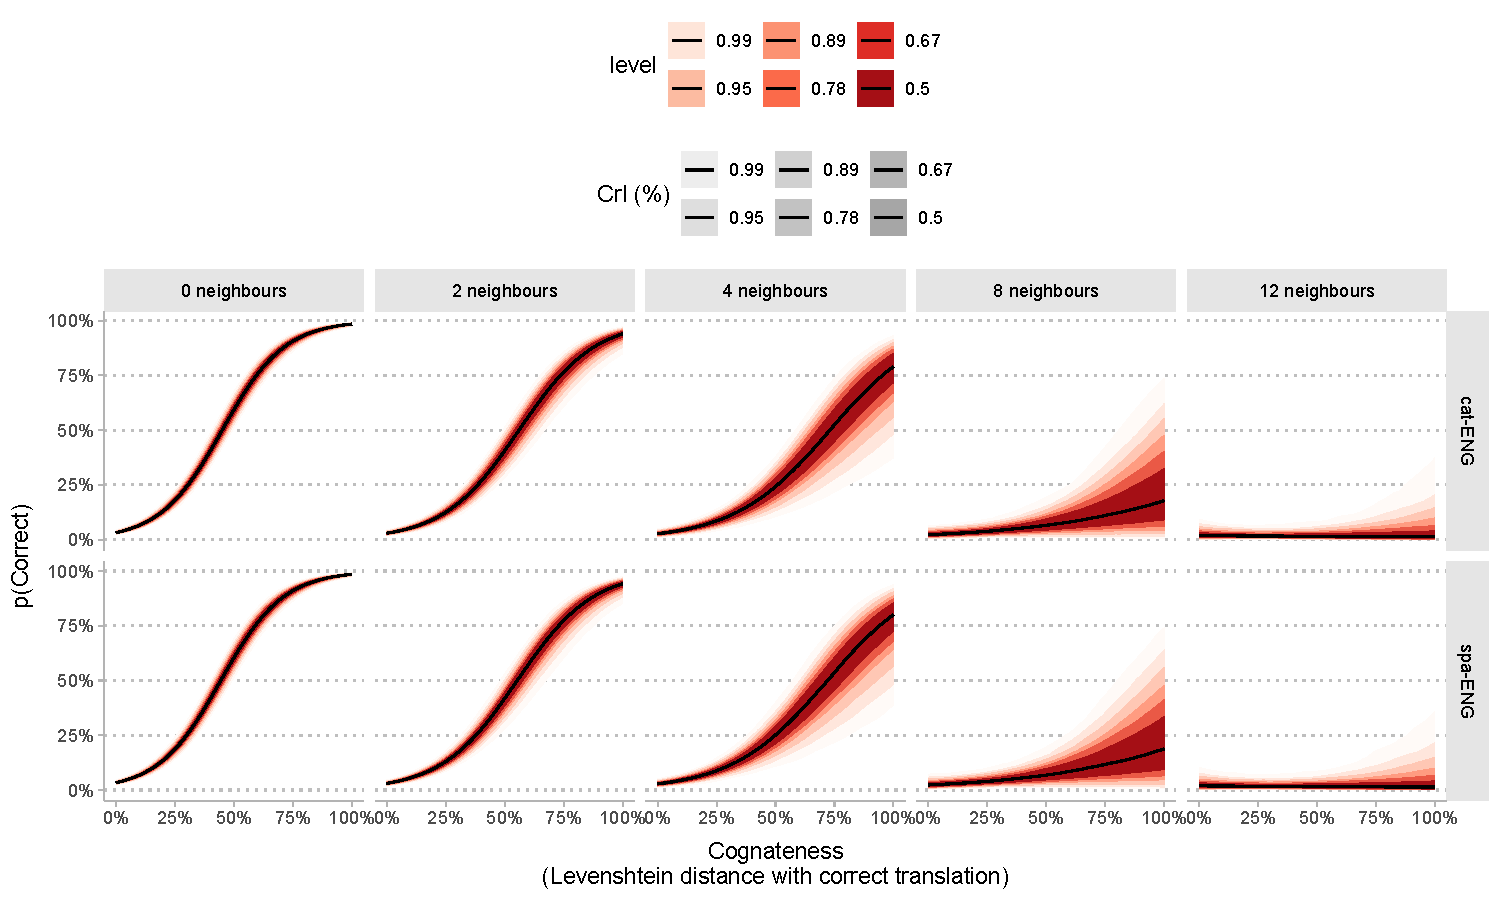
\includegraphics[keepaspectratio]{manuscript_files/figure-pdf/fig-epreds-3-1.pdf}}

}

\end{figure}%

\subsection{Discussion}\label{discussion-2}

Experiment 3 was a conceptual replication of Experiment 1 in which we
gathered additional information about English native participants' prior
familiarity with the meaning of the Catalan and Spanish words presented.
After each trial, participants reported whether they had prior knowledge
about the word meaning, and how confident they were about such
information in a numeric scale from 0 to 7. To control for the effect of
participants' prior knowledge about form-meaning mappings, we excluded
from the analyses those words in which participants reported such prior
knowledge. We found equivalent results to those in Experiment 1,
indicating that participants' surprisingly good performance in the
translation elicitation task was not due to being familiar with the
meaning of words they were presented with.

\section{General discussion}\label{general-discussion}

The present work explored the lexical processing bases of homophonic
translation, a phenomenon in which listening to speech in a
non-native---perhaps unfamiliar---language leads to the activation of
lexical representations in the native language, without necessarily
preserving the meaning. We investigated how phonological similarity and
its interaction with phonological neighbourhood density impact the
dynamics of lexical activation and selection during non-native word
processing. We designed a translation elicitation task in which
participants listened to individual words in a non-native, unfamiliar
language. After listening to each word, participants were asked to
provide their best-guess translation for each word in their native
language. In Experiment 1, British English-native adults listened to a
list of words in Catalan or Spanish. Participants reported no prior
familiarity with Catalan, Spanish, or any other Romance language, yet
provided accurate translations for words that shared some degree of
phonological similarity with their correct English translation. We
calculated phonological similarity between word pairs as the Levenshtein
similarity between the X-SAMPA transcription of their phonological forms
(see \citeproc{ref-floccia2018introduction}{Floccia et al., 2018} for a
similar approach). Using this measure, we found that participants were
able to exploit the phonological similarity between the presented words
and their correct translation, even when both words-forms shared few
phonemes. This points to listeners accommodating non-native phonological
forms to their native phoneme inventory, resulting in the activation of
native lexical representations.

Experiment 2 was aimed at extending our findings to a population of
participants whose native language was typologically closer to the
unfamiliar language presented. We tested a group of Spanish native
adults who listened to a list of Catalan words. Again, participants
reported no prior familiarity with Catalan, or any other Romance
language other than Spanish. In line with the results with English
natives, we found an interaction between phonological similarity and
phonological neighbourhood size. Spanish natives in Experiment 2
exploited phonological similarity more strongly than English natives in
Experiment 1: the association between phonological similarity and the
probability of correct translation was stronger in Experiment 2,
compared to in Experiment 1.

Experiment 3 was a replication of Experiment 1, in which we collected
additional information about participants' prior familiarity with the
presented Catalan and Spanish words. This follow-up experiment was
designed to address concerns that participants in Experiments 1 and 2
might have managed to provide correct translations for some words thanks
to having prior experience with those words. The design of Experiment 3
was closely modelled after Experiment 1, except that after providing
their response in each trial, participants reported whether they had
previous knowledge of the presented word. After removing responses where
participants reported prior knowledge about the meaning of the presented
Catalan or Spanish word, we ran the same analyses as in Experiment 1,
and found parallel results. Overall, our results suggest that
participants were able to rely on the phonological similarity between
the presented Catalan and Spanish words and their correct translation to
guide word recognition in an unfamiliar language.

Future studies may consider comparing the suitability of other measures
of phonological similarity that take into account finer-grained phonetic
or prosodic cues present in the acoustic signal presented to
participants. Phonological transcriptions like X-SAMPA are abstract
representations that ignore non-phonological contrasts (e.g., phones),
and consider different symbols as completely different phonemes,
disregarding the fact that some phonemes share more phonetic features
than others. Additionally, prosodic cues such as lexical stress, which
our measure of phonological similarity does not include, might also
provide participants further information about the correct translation
of the presented word-forms. Altogether, it is likely that participants
in the present study were able to exploit additional cues in the
acoustic signal to provide correct translations. Future studies may
explore the relative contribution of such cues in the occurrence of
homophonic translation. Overall, the present study provides some
insights into the role of phonological similarity in the auditory
presentation of words in an unfamiliar language.

Our findings also suggest that the facilitation effect of phonological
similarity was moderated by phonological neighbourhood density. This is
in line with previous studies suggesting that the presence of
(high-frequency) phonological neighbours interferes with the lexical
selection in word comprehension tasks (e.g.,
\citeproc{ref-dufour2010phonological}{Dufour \& Frauenfelder, 2010};
\citeproc{ref-grainger1990word}{Grainger, 1990};
\citeproc{ref-luce1998recognizing}{Luce \& Pisoni, 1998};
\citeproc{ref-vitevitch1998words}{Vitevitch \& Luce, 1998};
\citeproc{ref-vitevitch1999probabilistic}{Vitevitch \& Luce, 1999}). Our
translation elicitation task can be understood as a particular instance
of an auditory word recognition task, in which the presented unfamiliar
words have the potential to activate phonological neighbours in
participants' lexicon. We calculated a measure of cross-linguistic
neighbourhood size by counting, for each presented word the number of
phonologically related words (with a Levenshtein distance of one) in the
target language (English in Experiments 1 and 3, Spanish in Experiment
2). To account for the fact that competition between phonological
neighbours is sensitive to lexical frequency---high-frequency neighbours
produce stronger interference effects
(\citeproc{ref-dufour2010phonological}{Dufour \& Frauenfelder, 2010};
\citeproc{ref-luce1998recognizing}{Luce \& Pisoni, 1998})---we only
counted neighbours with a lexical frequency higher than the correct
translation. Using this measure, we found that participants' ability to
exploit phonological similarity to produce correct translations declined
as the number of phonological neighbours increased. This suggests that
listening to words in an unfamiliar language triggered similar
mechanisms of lexical activation and selection that listening to words
in a native language does. The generalisability of these findings can be
tested by increasing the repertoire of words involved in the translation
elicitation task. In Experiments 1 to 3, participants answered to a
maximum of 105 words. All words had high frequency and low
age-of-acquisition. To better characterise the factors that guide
listeners' ability to match words from an unfamiliar language with words
in their native language lexicon, words with varying levels of
difficulty should be included in future studies.

A comparison between the results in Experiments 1 and 2 suggested that
the performance of Spanish participants translating Catalan was more
resilient to the interfering effects of phonological neighbourhood
density than the performance of English participants translating Catalan
or Spanish. As highlighted before, Catalan and Spanish (both Romance
languages) are typologically closer to each other than to English (a
Germanic language). Catalan and Spanish share a higher proportion of
cognates than Catalan and English, or Spanish and English. Overall, our
findings suggest that the typological distance between the presented and
target language is associated with a more robust facilitation effect of
phonological similarity.

The specific mechanisms behind this effect are unclear. One possibility
is that there were subphonemic features of similarity between Catalan
and Spanish words that were not adequately captured by our relatively
coarse measure of similarity. Phonological transcriptions like X-SAMPA
are abstract representations that ignore non-phonological contrasts
(e.g., phones), and consider different symbols as completely different
phonemes, disregarding the fact that some phonemes share more phonetic
features than others. Additionally, prosodic cues such as lexical
stress, which our measure of phonological similarity does not include,
might also provide participants with further information about the
correct translation of the presented word-forms. There may be more of
these subphonemic cues available between the typologically close Spanish
and Catalan than between the more distant English and Spanish, or
English and Catalan. In addition, it remains to be tested whether the
effect of typological distance is linear (i.e., robustness of
facilitation increases linearly with typological distance),
proportional, and whether other close or distant language pairs show the
same pattern of results. Future studies may consider comparing the
suitability of other measures of phonological similarity that take into
account finer-grained phonetic or prosodic cues present in the acoustic
signal, and explore the relative contribution of such cues in the
occurrence of homophonic translation.

In summary, the present paper provides insights into the processing
mechanisms underlying homophonic translation. English and Spanish native
adults were tested in a translation elicitation task in which they had
to guess the English or Spanish translation of a series of words in an
unfamiliar language. Participants successfully exploited phonological
similarity between the presented words and their correct translations to
provide correct answers. Participants' performance in the task only
benefited from phonological similarity when the presented word had few
higher-frequency phonological neighbours in the target language.
Finally, the facilitation effect of phonological similarity was stronger
in the Spanish native participants, who translated words from a
typologically closer language than English participants. Overall, the
findings presented in the present paper suggest that the processing of
words in a non-native, unfamiliar language recruits mechanisms of
lexical activation, selection, and interference parallel to those
recruited by listening to words in a native language.

\section*{References}\label{references}
\addcontentsline{toc}{section}{References}

\phantomsection\label{refs}
\begin{CSLReferences}{1}{0}
\bibitem[\citeproctext]{ref-briusov1911ot}
Briusov, V. Y. (1911). \emph{Ot perevodchika}. Skorpion.

\bibitem[\citeproctext]{ref-broersma2021praat}
Broersma, P., \& Weenink, D. (2021). \emph{Praat: Doing phonetics by
computer {[}{Computer} program{]}} (Version 6.1.54).
\url{http://www.praat.org/}

\bibitem[\citeproctext]{ref-burkner2017brms}
Bürkner, P.-C. (2017). Brms: {An R} package for {Bayesian} multilevel
models using {Stan}. \emph{Journal of Statistical Software},
\emph{80}(1), 1--28.

\bibitem[\citeproctext]{ref-carpenter2017stan}
Carpenter, B., Gelman, A., Hoffman, M. D., Lee, D., Goodrich, B.,
Betancourt, M., Brubaker, M., Guo, J., Li, P., \& Riddell, A. (2017).
Stan: {A} probabilistic programming language. \emph{Journal of
Statistical Software}, \emph{76}(1), 1--32.

\bibitem[\citeproctext]{ref-cervantes}
Cervantes, M. de, \& Grossman, E. (2002). First part of the ingenious
nobleman don quixote of la mancha. \emph{Conjunctions}, \emph{38},
207--225. \url{http://www.jstor.org/stable/24518146}

\bibitem[\citeproctext]{ref-dembeck2015oberflachenubersetzung}
Dembeck, T. (2015). Oberfl{ä}chen{ü}bersetzung: The poetics and cultural
politics of homophonic translation. \emph{Critical Multilingualism
Studies}, \emph{3}(1), 7--25.

\bibitem[\citeproctext]{ref-dufour2010phonological}
Dufour, S., \& Frauenfelder, U. H. (2010). Phonological neighbourhood
effects in french spoken-word recognition. \emph{Quarterly Journal of
Experimental Psychology}, \emph{63}(2), 226--238.

\bibitem[\citeproctext]{ref-dufour2003lexical}
Dufour, S., \& Peereman, R. (2003). Lexical competition in phonological
priming: {Assessing} the role of phonological match and mismatch lengths
between primes and targets. \emph{Memory \& Cognition}, \emph{31},
1271--1283.

\bibitem[\citeproctext]{ref-dupoux1999epenthetic}
Dupoux, E., Kakehi, K., Hirose, Y., Pallier, C., \& Mehler, J. (1999).
Epenthetic vowels in japanese: A perceptual illusion? \emph{Journal of
Experimental Psychology: Human Perception and Performance},
\emph{25}(6), 1568.

\bibitem[\citeproctext]{ref-efimova2018homophonic}
Efimova, N. N., Ruzhnikova, M. L., \& Violina, M. I. (2018). Homophonic
translation as humpty-dumpty's choice. \emph{SHS Web of Conferences},
\emph{50}, 01049.

\bibitem[\citeproctext]{ref-floccia2018introduction}
Floccia, C., Sambrook, T. D., Delle Luche, C., Kwok, R., Goslin, J.,
White, L., Cattani, A., Sullivan, E., Abbot-Smith, K., Krott, A., et al.
(2018). I: {Introduction}. \emph{Monographs of the Society for Research
in Child Development}, \emph{83}(1), 7--29.

\bibitem[\citeproctext]{ref-gasparov2006semen}
Gasparov, M. L. (2006). \emph{Semen kirsanov}. Akademicheskij proekt.

\bibitem[\citeproctext]{ref-goldinger1989priming}
Goldinger, S. D., Luce, P. A., \& Pisoni, D. B. (1989). Priming lexical
neighbors of spoken words: {Effects} of competition and inhibition.
\emph{Journal of Memory and Language}, \emph{28}(5), 501--518.
\url{https://doi.org/10.1016/0749-596X(89)90009-0}

\bibitem[\citeproctext]{ref-grainger1990word}
Grainger, J. (1990). Word frequency and neighborhood frequency effects
in lexical decision and naming. \emph{Journal of Memory and Language},
\emph{29}(2), 228--244.

\bibitem[\citeproctext]{ref-hamburger1996phonological}
Hamburger, M., \& Slowiaczek, L. M. (1996). Phonological priming
reflects lexical competition. \emph{Psychonomic Bulletin \& Review},
\emph{3}(4), 520--525.

\bibitem[\citeproctext]{ref-kruschke2018bayesian}
Kruschke, J. K., \& Liddell, T. M. (2018). The {Bayesian New
Statistics}: {Hypothesis} testing, estimation, meta-analysis, and power
analysis from a {Bayesian} perspective. \emph{Psychonomic Bulletin \&
Review}, \emph{25}, 178--206.

\bibitem[\citeproctext]{ref-levenshtein1966binary}
Levenshtein, V. I. (1966). Binary codes capable of correcting deletions,
insertions, and reversals. \emph{Soviet Physics Doklady}, \emph{10},
707--710.

\bibitem[\citeproctext]{ref-levick2016translating}
Levick, T. (2016). Translating homophonic wordplay in patrick goujon's
moi non: A case study. \emph{Sound/Writing: On Homophonic Translation}.

\bibitem[\citeproctext]{ref-luce1998recognizing}
Luce, P. A., \& Pisoni, D. B. (1998). Recognizing spoken words: {The}
neighborhood activation model. \emph{Ear and Hearing}, \emph{19}(1), 1.

\bibitem[\citeproctext]{ref-luce1990similarity}
Luce, P. A., Pisoni, D. B., \& Goldinger, S. D. (1990). \emph{Similarity
neighborhoods of spoken words.}

\bibitem[\citeproctext]{ref-marian2012clearpond}
Marian, V., Bartolotti, J., Chabal, S., \& Shook, A. (2012).
\emph{{CLEARPOND}: {Cross-linguistic} easy-access resource for
phonological and orthographic neighborhood densities}.

\bibitem[\citeproctext]{ref-otake2007interlingual}
Otake, T. (2007). Interlingual near homophonic words and phrases in L2
listening: Evidence from misheard song lyrics. \emph{Proceedings of the
16th International Congress of Phonetic Sciences (ICPhS 2007)},
777--780.

\bibitem[\citeproctext]{ref-otwinowska2019more}
Otwinowska, A., \& Szewczyk, J. M. (2019). The more similar the better?
Factors in learning cognates, false cognates and non-cognate words.
\emph{International Journal of Bilingual Education and Bilingualism}.

\bibitem[\citeproctext]{ref-peirce2019psychopy2}
Peirce, J., Gray, J. R., Simpson, S., MacAskill, M., Höchenberger, R.,
Sogo, H., Kastman, E., \& Lindeløv, J. K. (2019). {PsychoPy2}:
{Experiments} in behavior made easy. \emph{Behavior Research Methods},
\emph{51}(1), 195--203. \url{https://doi.org/10.3758/s13428-018-01193-y}

\bibitem[\citeproctext]{ref-peperkamp2008perceptual}
Peperkamp, S., Vendelin, I., \& Nakamura, K. (2008). On the perceptual
origin of loanword adaptations: Experimental evidence from japanese.
\emph{Phonology}, \emph{25}(1), 129--164.

\bibitem[\citeproctext]{ref-pilshchikov2016semiotics}
Pilshchikov, I. (2016). The semiotics of phonetic translation.
\emph{Studia Metrica Et Poetica}, \emph{3}(1), 53--104.

\bibitem[\citeproctext]{ref-rcoreteam2013language}
R Core Team. (2013). \emph{R: {A Language} and {Environment} for
{Statistical Computing}}. R Foundation for Statistical Computing.
\url{http://www.R-project.org/}

\bibitem[\citeproctext]{ref-schad2020capitalize}
Schad, D. J., Vasishth, S., Hohenstein, S., \& Kliegl, R. (2020). How to
capitalize on a priori contrasts in linear (mixed) models: {A} tutorial.
\emph{Journal of Memory and Language}, \emph{110}, 104038.

\bibitem[\citeproctext]{ref-schepens2012distributions}
Schepens, J., Dijkstra, T., \& Grootjen, F. (2012). Distributions of
cognates in {Europe} as based on {Levenshtein} distance.
\emph{Bilingualism: Language and Cognition}, \emph{15}(1), 157--166.

\bibitem[\citeproctext]{ref-van2014stringdist}
van der Loo, M. P. J. (2014). The stringdist package for approximate
string matching. \emph{The R Journal}, \emph{6}(1), 111--122.
\url{https://CRAN.R-project.org/package=stringdist}

\bibitem[\citeproctext]{ref-van2014subtlex}
Van Heuven, W. J., Mandera, P., Keuleers, E., \& Brysbaert, M. (2014).
{SUBTLEX-UK}: {A} new and improved word frequency database for {British
English}. \emph{Quarterly Journal of Experimental Psychology},
\emph{67}(6), 1176--1190.

\bibitem[\citeproctext]{ref-vitevitch2006clustering}
Vitevitch, M. (2006). The clustering coefficient of phonological
neighborhoods influences spoken word recognition. \emph{The Journal of
the Acoustical Society of America}, \emph{120}(5), 3252--3252.
\url{https://doi.org/10.1121/1.4788314}

\bibitem[\citeproctext]{ref-vitevitch1998words}
Vitevitch, M. S., \& Luce, P. A. (1998). When words compete: Levels of
processing in perception of spoken words. \emph{Psychological Science},
\emph{9}(4), 325--329.

\bibitem[\citeproctext]{ref-vitevitch1999probabilistic}
Vitevitch, M. S., \& Luce, P. A. (1999). Probabilistic {Phonotactics}
and {Neighborhood Activation} in {Spoken Word Recognition}.
\emph{Journal of Memory and Language}, \emph{40}(3), 374--408.
\url{https://doi.org/10.1006/jmla.1998.2618}

\bibitem[\citeproctext]{ref-weber2004lexical}
Weber, A., \& Cutler, A. (2004). Lexical competition in non-native
spoken-word recognition. \emph{Journal of Memory and Language},
\emph{50}(1), 1--25.

\bibitem[\citeproctext]{ref-wickham2019welcome}
Wickham, H., Averick, M., Bryan, J., Chang, W., McGowan, L. D.,
François, R., Grolemund, G., Hayes, A., Henry, L., Hester, J., Kuhn, M.,
Pedersen, T. L., Miller, E., Bache, S. M., Müller, K., Ooms, J.,
Robinson, D., Seidel, D. P., Spinu, V., \ldots{} Yutani, H. (2019).
Welcome to the tidyverse. \emph{Journal of Open Source Software},
\emph{4}(43), 1686. \url{https://doi.org/10.21105/joss.01686}

\end{CSLReferences}

\appendix

\section{}\label{}

\subsection{Appendix 1: Model diagnostics}\label{apx-diagnostics}

One way to diagnose the behaviour of Hamiltonian Monte Carlot (HMC, the
algorithm used by Stan to explore the posterior distribution of a model)
is to check whether the MCMC chains have converged.
\textbf{?@fig-appendix-diagnostics} shows the values sampled by the MCMC
chains of each of the fixed coefficients of each model reported in the
manuscript. Evidence of chain convergence is provided by the same region
of values being sampled across the final interations of the chain, as it
is the case for the three models depicted.

\begin{figure}[H]

\caption{Traceplots of fixed regression coefficients of models in
Experiments 1, 2, and 3.}

{\centering \pandocbounded{\includegraphics[keepaspectratio]{manuscript_files/figure-pdf/apxfig-appendix-diagnostics-1.pdf}}

}

\end{figure}%

\section{}\label{}

\subsection{Appendix 2: Pooled analyses of Experiments 1 and
3}\label{apx-pooled}

Across Experiments 1 and 3, we found strong evidence that participants
efficiently exploited phonological similarity to provide accurate
translations for words in an unfamiliar language, provided that few
phonological neighbours of higher lexical frequency were present.
\textbf{?@fig-coefs} summarizes the posterior distribution of the
regression coefficients of the models in Experiments 1 to 3.

\begin{figure}[H]

\caption{Regression coefficients across Experiments 1, 2, and 3.}

{\centering \pandocbounded{\includegraphics[keepaspectratio]{manuscript_files/figure-pdf/apxfig-coefs-1.pdf}}

}

\end{figure}%






\end{document}